\documentclass[12pt]{article}

\usepackage{amsmath}
\usepackage{amsfonts}
\usepackage{amssymb}
\usepackage{amsthm}
\usepackage{centernot}
\usepackage{tikz}
\usepackage{hyperref}
\usepackage[capitalise,poorman,nameinlink]{cleveref}


% TODO Remove debug
\newcommand{\mlabel}[1]{\label{#1}\marginpar{\tiny\texttt{[\detokenize{#1}]}}}

\newcommand{\myskip}{\bigskip\noindent}

\newcommand{\typeeq}{\simeq} % Type equal ~_
\newcommand{\ntypeeq}{\not\typeeq} % Not type equal
\newcommand{\eqclass}[1]{[{#1}]} % only used to be able to write $[]$ inside [...]

\newcommand{\vald}{\mathsf{D}} % Directory value
\newcommand{\valdi}{\mathsf{D}_1}
\newcommand{\valdii}{\mathsf{D}_2}
\newcommand{\valfx}{\mathsf{F}} % File value
\newcommand{\valf}{\mathsf{F}_i} % File value
\newcommand{\valff}{\mathsf{F}_j} % File value
\newcommand{\empt}{\ominus} % Empty value
\newcommand{\valv}{v} % Any value
\newcommand{\valvy}{::v_Y::} % TODO DELETE
\newcommand{\valvw}{::v_W::} % TODO DELETE

\newcommand{\setfs}{\mathbb{F}} % TODO DELETE Set of filesystems
\newcommand{\setv}{\mathbb{V}} % Set of values
\newcommand{\setn}{\mathbb{N}} % Set of nodes / paths
\newcommand{\setd}{[\vald]} % Set of directory values

\newcommand{\fsreplacement}[3]{{#1}_{[{#2}\rightarrow{#3}]}} % {FS}{node}{newvalue}

\newcommand{\parent}{\mathord{\shortuparrow}} % parent function symbol
\newcommand{\parentf}[1]{\parent({#1})} % parent function
\newcommand{\fsbroken}{\bot} % value when command is not defined / broken FS value
\newcommand{\FS}{\Phi} % a filesystem
\newcommand{\aFS}{\,\FS} % a filesystem preceded by something applied to it
\newcommand{\nn}{n'} % parent node
\newcommand{\pn}{\parentf{n}} % parent node
\newcommand{\Tsign}{\tau} % type-equivalent class mapping
\newcommand{\T}[1]{{#1}_\Tsign} % type-equivalent class mapping
\newcommand{\TA}{\T{A}}
\newcommand{\TB}{\T{B}}
\newcommand{\TC}{\T{C}}
\newcommand{\TS}{\T{S}}

\newcommand{\cbrk}{\epsilon_\varnothing} % 'break' / empty command

\newcommand{\caa}[2]{::\langle{[#1],[#2]}\rangle::} % Command template
\newcommand{\caaa}[3]{\langle{[#1],#2,#3}\rangle}
\newcommand{\caaaa}[3]{\langle{[#1],#2,#3}\rangle}

\newcommand{\cbb}{\caa{::\empt}{\empt}} % TODO delete
\newcommand{\cbf}{\caa{::\empt}{\valf}} % TODO delete
\newcommand{\cbd}{\caa{::\empt}{\vald}} % TODO delete
\newcommand{\cfb}{\caa{::\valf}{\empt}} % TODO delete
\newcommand{\cff}{\caa{::\valf}{\valf}} % TODO delete
\newcommand{\cfd}{\caa{::\valf}{\vald}} % TODO delete
\newcommand{\cdb}{\caa{::\vald}{\empt}} % TODO delete
\newcommand{\cdf}{\caa{\vald}{\valfx}} % TODO delete
\newcommand{\cdd}{\caa{::\vald}{\vald}} % TODO delete

\newcommand{\cbba}[1]{\caaa{\empt}{\empt}{#1}}
\newcommand{\cbfa}[1]{\caaa{\empt}{\valfx}{#1}}
\newcommand{\cbda}[1]{\caaa{\empt}{\vald}{#1}}
\newcommand{\cfba}[1]{\caaa{\valfx}{\empt}{#1}}
\newcommand{\cfda}[1]{\caaa{\valfx}{\vald}{#1}}
\newcommand{\cdba}[1]{\caaa{\vald}{\empt}{#1}}
\newcommand{\cdfa}[1]{\caaa{\vald}{\valfx}{#1}}
\newcommand{\cdda}[1]{\caaa{\vald}{\vald}{#1}}

\newcommand{\cxy}{\caa{x}{y}} % TODO delete
\newcommand{\cxyaa}[1]{\caaa{x}{y}{#1}}
\newcommand{\cxynv}{\caaa{x}{y}{n}}
\newcommand{\cxynnv}{\caaa{x}{y}{\nn}}
\newcommand{\cxypnv}{\caaa{x}{y}{\pn}}
\newcommand{\cxw}{\caa{x}{w}} % TODO delete
\newcommand{\cxwnv}{\caaa{x}{w}{n}}
\newcommand{\czw}{\caa{z}{w}} % TODO delete
\newcommand{\czwnv}{\caaa{z}{w}{n}}
\newcommand{\czwnnv}{\caaa{z}{w}{\nn}}
\newcommand{\czwpnv}{\caaa{z}{w}{\pn}}
\newcommand{\czwmv}{\caaa{z}{w}{m}}
\newcommand{\cqrnv}{\caaa{q}{r}{n}}
\newcommand{\cqrmv}{\caaa{q}{r}{m}}
\newcommand{\cqrov}{\caaa{q}{r}{o}}

% \newcommand{\cc}{\mathbin{\circ}} % Command / sequence concatenation
\newcommand{\compcent}[1]{\vcenter{\hbox{$#1\circ$}}}
\newcommand{\cc}{\mathbin{\mathchoice
  {\compcent\scriptstyle}{\compcent\scriptstyle}
  {\compcent\scriptscriptstyle}{\compcent\scriptscriptstyle}}}

\newcommand{\descendant}{\prec}
\newcommand{\descendantEq}{\preceq}
\newcommand{\ancestor}{\succ}
\newcommand{\ancestorEq}{\succeq}

\newcommand{\eqext}{\sqsubseteq} % extended by "[="
\newcommand{\eqnrw}{\sqsupseteq} % extends "]="
\newcommand{\strext}{\sqsubset} % extended by (strict) "["
\newcommand{\strnrw}{\sqsupset} % extends (strict) "]"
\newcommand{\nequiv}{\not\equiv}

\newcommand{\indep}{\mathrel{\wr\wr}} % Independent commands, sequences
\newcommand{\unrel}{\indep} % Incomparable (unrelated) nodes
\newcommand{\nindep}{\mathrel{\centernot{\wr\wr}}} % not \indep
\newcommand{\nunrel}{\nindep} % not \unrel

\newcommand{\worksmsign}{\vartriangleleft} % works-more sign "<"
\newcommand{\worksmeqsign}{\trianglelefteq} % works-more-eq sign "<="
\newcommand{\worksm}[2]{{#1}\worksmeqsign{#2}} % works-more-eq "<="
\newcommand{\worksmxb}[2]{\worksm{#1}{\{{#2}\}}}
\newcommand{\worksmbx}[2]{\worksm{\{{#1}\}}{#2}}
\newcommand{\worksmbb}[2]{\worksm{\{{#1}\}}{\{{#2}\}}}

\newcommand{\wrks}[1]{\cbrk\strext{#1}} % sequence works "["
\newcommand{\wrksx}[1]{{#1}\strnrw\cbrk} % sequence works (reverse order) "]"
\newcommand{\worksmnil}[1]{{\cbrk}\worksmsign{#1}} % set works "<"
\newcommand{\worksmnilb}[1]{{\cbrk}\worksmsign{\{{#1}\}}} % set works "<"

\newcommand{\emptyseq}{\lambda} % empty sequence

\newcommand{\ordersetsign}{\vec{P}}
\newcommand{\orderset}[1]{\ordersetsign({#1})}
\newcommand{\ordsign}{\vec{c}} % Set of commands with assumed order
\newcommand{\ords}[1]{\ordsign\{{#1}\}} % Set of commands with assumed order, {}
\newcommand{\ordp}[1]{\ordsign\,({#1})} % Set of commands with assumed order, ()

\newcommand{\seqset}[1]{\mathcal{#1}} % Set of sequences
\newcommand{\sqs}[1]{\seqset{#1}}

\newcommand{\recchar}[3]{{#1}^{#3}_{\mathcal{R}|{#2}}}
\newcommand{\reca}{\recchar{A}{B}{}} % Reconciled from A
\newcommand{\recb}{\recchar{B}{A}{}} % Reconciled from B

\newcommand{\mynegsp}{\nobreak\hspace{-1pt plus 1pt}\nobreak}
\newcommand{\acbnp}{A\mynegsp\cap\mynegsp B} % A^B
\newcommand{\acb}{\ordp{\acbnp}} % c(A^B)
\newcommand{\acbi}{{\T{\acb}}^{-1}} % c(A^B)T-1
\newcommand{\ambnp}{A\mynegsp\setminus\mynegsp B}
\newcommand{\amb}{\ordp{\ambnp}}
\newcommand{\bmanp}{B\mynegsp\setminus\mynegsp A}
\newcommand{\bma}{\ordp{\bmanp}}

\newcommand{\Dom}[1]{\textrm{Dom}({#1})}

\newcommand{\whr}{\mathrel{|}}

\newcommand{\rot}[3]{#3#2#1} % Rotate
\newcommand{\undersc}{\texttt{\detokenize{_}}}


\theoremstyle{definition}
\newtheorem{mydefaux}{Definition}
\crefname{mydefaux}{Definition}{Definitions}
\newenvironment{mydef}{\renewcommand\qedsymbol{$\blacktriangleright$}\pushQED{\qed}\mydefaux}{\popQED\endmydefaux}

\theoremstyle{plain}
\newtheorem{myax}{Rule**}
\crefname{myax}{Rule**}{Rules**} % TODO delete

\crefname{rulecounter}{Rule}{Rules}

\theoremstyle{plain}
\newtheorem{mylem}{Lemma}
\crefname{mylem}{Lemma}{Lemmas}

\theoremstyle{plain}
\newtheorem{myth}{Theorem}
\crefname{myth}{Theorem}{Theorems}

\theoremstyle{plain}
\newtheorem{mycor}{Corollary}
\crefname{mycor}{Corollary}{Corollaries}

\theoremstyle{plain}
\newtheorem{myclm}{Claim}
\crefname{myclm}{Claim}{Claims}

\theoremstyle{plain}
\newtheorem{myaxproof}{Rule}
\crefname{myaxproof}{Rule}{Rules}


\title{Algebraic File Synchronization: Adequacy and Completeness}
\author{Elod Pal Csirmaz\\
\texttt{\rot{\rot{maz.}{csir}{ep}com}{@}{elod}}}
\date{}

\begin{document}
\maketitle
\begin{abstract}


With distributed computing and mobile applications,
synchronizing diverging replicas of data structures is a more and more common problem.
We use algebraic methods to reason about filesystem operations, 
and introduce a simplified definition of conflicting updates to filesystem trees.
We also define algorithms for update detection and reconciliation
and present rigorous proofs that they not only work as intended,
but also cannot be improved on.

To achieve this, we introduce a novel, symmetric set of filesystem commands
with higher information content,
which removes edge cases
and increases the predictive powers of our algebraic model.
We also present a number of generally useful classes and properties
of sequences of commands.

These results are often intuitive,
but providing exact proofs for them is far from trivial.
They contribute to our understanding of this special type of algebraic model,
and toward building more complete algebras
of filesystems 
and extending algebraic approaches to other data storage protocols.
They also form a theoretical basis for
specifying
and guaranteeing the error-free operation
of applications that implement an algebraic approach to synchronization.


\bigskip\noindent
{\bf Keywords:} % (4-6)
file synchronization,
algebraic approach,
distributed systems,
reconciliation,
data replication
% conflict detection,
% conflict resolution
% computer algebra

\bigskip\noindent
{\bf MSC classes:} % http://www.ams.org/mathscinet/msc/msc2010.html
08A70, % Applications of universal algebra in computer science
68M07, % Mathematical problems of computer architecture
68M14, % Distributed systems
68P05, % Data structures
68P20 % Information storage and retrieval
% 68N25         Operating systems

\bigskip\noindent
{\bf ACM classes:} % http://www.acm.org/about/class/ccs98-html
% (D) Software (D.4) Operating systems
D.4.3, % File systems management
% (E) Data
E.5, % Files
% (F) Theory of computation (F.2) ANALYSIS OF ALGORITHMS AND PROBLEM COMPLEXITY
F.2.2, % Nonnumerical Algorithms and Problems
% (G) Mathematics of Computing
G.2 % DISCRETE MATHEMATICS
% (H) Information Systems (H.3) INFORMATION STORAGE AND RETRIEVAL
% H.3.4 % Systems and Software

\end{abstract}

% section

\section{Introduction}

Synchronization of data structures
is a mechanism behind many services we take for granted today:
accessing and editing calendar events, documents and spreadsheets
on multiple devices, version control systems and
geographically distributed internet and web services that
guarantee a fast and responsive user experience.

In this paper we investigate a command-based approach
to synchronizing filesystem trees.
Presented with multiple copies (replicas) of the same filesystem that have been independently modified,
we regard the aim of the synchronizer to modify these replicas further
to make them as similar as possible.
The synchronization algorithm we describe
follows the two main steps described by Balasubramaniam and Pierce \cite{BP}:
update detection, where we identify modifications that have been applied to the replicas
since they diverged and represent them as sequences of commands;
and reconciliation, where we identify commands that can be propagated to other replicas and do so.
The remaining commands, which could not be propagated, represent conflicting updates;
resolving these requires a separate system or human intervention.

We extend significantly the results of the previous work done
with Prof. Norman Ramsey
on an algebraic approach to synchronization
\cite{NREC},
and add to the theoretical understanding
of synchronization by providing rigorous proofs that the algorithms
we describe work as intended
and offer a solution in our framework that cannot be improved on.

A central problem of command-based synchronizers 
during both update detection and reconciliation
is the ordering (scheduling) of commands.
If update detection is based on comparing the original state of the filesystem
to its new state, then we can easily collect a set of updates,
but we need to order these in a way that they could be applied
to the filesystem without causing an error 
(for example, a directory needs to be created before a file can be created under it).
Similarly, during reconciliation when we consider all the commands that
have been applied to the different replicas, we need to find a way of
merging these and creating a global ordering that we can apply
to the filesystems.
In fact, an insight in \cite{NREC} is that
if the ordering changes the effect of two commands,
then under certain circumstances they are not compatible and will give rise to conflicts.
Accordingly, in this paper command pairs, their commutativity and other properties
play a significant role.

In terms of the usual classification of synchronizers \cite{TSR, PV, SSH},
our approach to reconciliation is therefore operation-based as we investigate sets of commands,
while the update detection algorithm makes the full synchronizer 
similar to state-based synchronizers 
as its starting point is the states of the replicas themselves.
Moreover, our ordering algorithms only depend on properties of commands 
such as commutativity or idempotence,
and therefore they can be classified as semantic schedulers.
This is in opposition to syntactic scheduling, which uses 
the origin and the original temporal order of updates, 
and which may give rise to otherwise resolvable conflicts \cite{SSH}.
In general, ordering plays a central role in operation-based synchronizers.
We refer to an excellent survey by Saito and Shapiro of so-called optimistic replication algorithms \cite{SSH};
and, as examples,
to IceCube, where multiple orders are tested to find an acceptable one (\cite{KRSD}, see also \cite{MPV}),
or Bayou, where reconciling updates happens by redoing them in a globally determined order \cite{TTPDSH}.

The approach presented in this paper offers an improvement
over results described in \cite{NREC} in multiple ways.
We introduce a new set of commands that is symmetric and
captures more information about the updates,
and we restrict information content in directories
to exploit a further hidden symmetry in the command set.
These have the effect that reasoning about commands
becomes simpler as there are fewer edge cases,
and more powerful as 
predictions made by the reasoning are more accurate
due to the additional information content.
In fact, the new command set not only simplifies
our reconciliation algorithm, but also makes it maximal.
\cite{NREC} also lacked proofs that the update detection
and reconciliation algorithms it presented work as intended,
which we provide in the current paper.
While the results are intuitive, providing rigorous proofs
is far from trivial.
During the process, we define a number of auxiliary concepts
and show their relationships and the properties they possess.
In our view these construct a special algebraic model
that is worthy of interest and of further research on its own.

The paper is organized as follows.
%
We start by defining a model of filesystems and a set of commands
that we will use to describe updates and modifications in \cref{sec_def}.
%
This is followed by investigating the properties and behaviors
of command pairs in \cref{section_axioms}.
%
\Cref{sec_update} describes update detection and ordering filesystem commands.
The main result of this section is that under some simple conditions,
a set of filesystem commands executed in any feasible order leads
to the same changes in the filesystem.
%
The reconciliation and conflict detection algorithm is defined in
\cref{sec_rec}, which merges two sets of commands.
We then proceed to prove that the output of reconciliation
is correct in the sense that 
it can be applied to the replicas without causing an error,
and it is maximal
inasmuch as no further updates can be applied under any circumstances.
In order to be able to do this, we introduce
domains of sets of command sequences,
and show that it has a number of highly convenient properties.
%
\Cref{sec_multidir,sec_algebra,sec_conclusion}
describe extending our model to widen its applicability;
outline directions for further work on the introduced algebraic system,
and provide the conclusion.
%
We discuss related work, comparing our results to other research in \cref{sec_relatedwork},
while
\cref{axiom_proof} contains technical proofs for propositions on the behavior of command pairs.



\section{Definitions}\label{sec_def}


\subsection{The Filesystem}

We model a working filesystem
using a function $\FS$ with a set of nodes (filesystem paths) $\setn$ as its domain,
and a set of possible contents or values $\setv$ as its codomain.
\begin{mydef}[Filesystems, $\setn$, $\setv$ and $\setfs$]
\[ \FS: \setn \rightarrow \setv \]
In our model, $\setn$ 
serves as a namespace or ``skeleton'' for the filesystem.
It contains all possible nodes, including the ones 
where the file system contains no file or directory,
where in our model $\FS$ has a special value, $\empt\in\setv$.
We write $\setfs$ for the set of filesystems.
\end{mydef}

There is an ancestor / descendant relation defined over the nodes,
which arranges them in a (disjoint) union of rooted directed trees,
and which can be derived from the following $\parent$ function.
Tao et al. \cite{TSR} describe a similar filesystem model, although
they also model inodes and restrict the filesystem to just a single tree.
\begin{mydef}[$\parent$]
The partial function $\parent:\setn\nrightarrow\setn$
returns the parent node of $n$,
and is undefined if $n$ is the root of a tree.
\end{mydef}

\begin{mydef}[$n\descendant m$]
On $\setn$ the \emph{ancestor / descendant} relation is the
strict partial ordering determined by the $\parent$ function.
We write $n\descendant m$ if $n$ is the ancestor of $m$,
that is, $n=\parent^i(m)$ for some integer $i\ge 1$.
% or the path name of $n$ is an initial segment of that of $m$. 
We write $n\descendantEq m$ if $n\descendant m$ or $n=m$.
\end{mydef}

\begin{mydef}[$n\unrel m$]
We write $n\unrel m$, or $n$ and $m$ are \emph{incomparable}
iff $n\not\descendantEq m$ and $n\not\ancestorEq m$;
that is, incomparable nodes are on different branches or on different trees.
% none of the path names describing their location is an initial segment of the other.
\end{mydef}

Every working filesystem has a so-called \emph{tree property}, which means that
if the filesystem is not empty at a node, and the node has a parent,
then there must be a directory at the parent node.
To model this, we differentiate between files, directories, and the
empty value in $\setv$, and introduce the equivalence relation
$\typeeq$.

\begin{mydef}[Equivalence by type: $\typeeq$]
We write $v_1\typeeq v_2$ for $v_1,v_2\in\setv$ if $v_1$ and $v_2$ are both files,
are both directories, or are both $\empt$.
% In other words, if $\setf$ is the set of file values and $\setd$ is the set of directories, then
% with $\{\empt\}$ they form a partition of $\setv$:
% \[ \setv/{\typeeq} = \{\setd,\setf,\{\empt\}\}. \]
\end{mydef}

As usual, we write $[v]$ for the equivalence class of $v$, which represents its type.
We also consider metadata to be part of the values in $\setv$.

The formal definition of the tree property is therefore
\begin{mydef}[Tree property]
\[ \forall n\in\setn, \FS\in\setfs: \FS(n) \neq \empt \Longrightarrow \FS(\parent(n)) \in \setd \]
where $\parent(n)$ is defined, and where $\setd\subset\setv$ is the set of directories.
\end{mydef}

To avoid the proliferation of edge cases, we will furthermore suppose that
$|\setd|=1$, that is, apart from their location, all directories are equal;
and use $\vald$ to denote the single value of the directory type.
In appendix TODO we describe why it can be a sensible choice
for actual synchronizers, and we also present an encoding that makes it possible
to extend our results to the $|\setd|>1$ case.

%% TODO
% % To model this, in $\setv$ we select another special value
% % to represent directories, as we assume that apart from their location
% % in the filesystem, all directories are equal.
% % We do this because, as Bill Zissimopoulos pointed 
% % out \cite{BZ},
% % we often do not want to consider metadata stored in
% % directories (e.g. permission settings) during synchronization,
% % as these are not generally understood well by users,
% % and, if needed, conflict resolution on these settings can be easily automated.
% % We will also see that this assumption makes it possible
% % to define a maximal reconciliation algorithm.


% This means that as we move down from the root of a tree of nodes,
% the types of values we encounter in the filesystem can only change according to the
% transition diagram in \cref{fig_transition}, from directories ($\cchard$) to files ($\ccharf$)
% to empty nodes ($\ccharb$).
% 
% \begin{figure}[htb]
% \begin{center}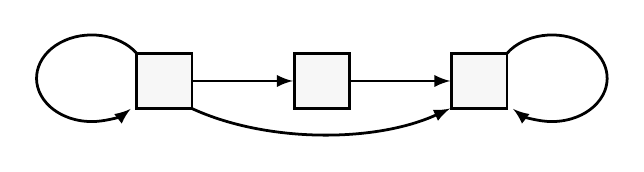
\begin{tikzpicture}
 [line width=1pt, bend angle=45,
 sq/.style={rectangle,inner sep=3pt, minimum size=7mm,
fill=black!3,draw=black}]
\node[sq] (dnode) at (0,0) {$\cchard$};
\node[sq] (fnode) at (2,0) {$\ccharf$};
\node[sq] (bnode) at (4,0) {$\ccharb$};
\draw[-latex] (dnode) -- (fnode);
\draw[-latex] (fnode) -- (bnode);
\draw[-latex] (-0.35,  0.35) arc(35:315:0.7cm and 0.55cm);
\draw[-latex] ( 4.35,  0.35) arc(145:-135:0.7cm and 0.55cm);
\draw[-latex] ( 0.35, -0.35) arc(230:310:2.55cm and 1.4cm);
\end{tikzpicture}\end{center}
% \caption{Transitions between types of values from the root of a tree in a filesystem}\label{fig_transition}
% \end{figure}

In this paper, $\FS$ and $\GS$ denote filesystems,
and $n$, $m$ and $o$ are nodes in $\setn$.
We write $\valf$ for an arbitrary file value. % element in $\setf$.




\subsection{Commands on Filesystems}

Next, we define commands on filesystems.
As described above, we aim to select a set of commands
that captures as much information
about the operations as possible, and is also symmetric.
We start by summarizing our reasons for doing so.

% What is encoded in a command?

Let us consider what kind of information is usually encoded in filesystem operations.
A minimal set of commands, based on the most frequent tools implemented by filesystems,
may be the following, where 
$n\in\setn$ and $\valv\in\setv$ (but $\valv\neq\empt$):
\begin{itemize}
\item \textit{create}$(n,\valv$), which creates a file or directory ($\valv$) at $n$
where the file system contains no file or directory ($\empt$);
\item \textit{edit}$(n,\valv)$, which replaces the earlier file or directory at $n$ with $\valv$;
\item \textit{remove}$(n)$, which removes the file or directory at $n$, and replaces it with $\empt$.
\end{itemize}
Regarding their output, that is, the state of the filesystem at $n$
after applying the command,
we know that after \textit{create} or \textit{edit,} $\FS(n)\neq\empt$, whereas after \textit{remove,}
$\FS(n)$ will be $\empt$. 
However, from \cite{NREC} and \cite{CBNR} we know that a useful set of axioms
will in some cases need to distinguish between, for example,
\textit{edit}s that result in directories (\textit{edit}$(n,\vald)$) and
ones that result in files (\textit{edit}$(n,\valf)$), and treat them as separate commands,
as their behaviors are quite different when combined with other commands.
Indeed, Bill Zissimopoulos' work
demonstrated \cite{BZ}
that extending this distinction to more commands ultimately simplifies
the definition of conflicting commands, as our model will then able to predict the behavior of commands
more precisely.

Notice, however, that the commands listed above also encode some information about 
their input, the state of the filesystem
before the command is applied. In particular, \textit{create}$(n,\valv)$ requires that there are no files
or directories at $n$, while \textit{edit}$(n,\valv)$ and \textit{remove}$(n)$ require the opposite.
This creates an arbitrary asymmetry where
there is now more information available about their output than about their input.
As, based on the above, we expect that encoding more information in the commands
results in a model with greater predictive powers,
and in order to resolve this asymmetry, 
we propose a set of commands that encode
the type of the input value $\FS(n)$ as well.
(Some real-life filesystem commands like \textit{rmdir} do this already.)
Because the success of failure of commands depends on types of values,
it is not necessary to encode the actual input value.

% Definition
% Break / empty command

We model filesystem commands as partial functions 
that map filesystems to filesystems, but which
are only defined where the commands succeed.
As usual, if the function is not defined, we say that that it returns the bottom element, $\fsbroken$,
or that it \emph{breaks} the filesystem.
We describe a filesystem commands using its input, output, and
the node it is applied to.

\begin{mydef}[Filesystem commands]
Filesystem commands are partial endofunctions on filesystems,
which are not defined on filesystems where they return an error.
The commands are represented using triplets of the form
\[ \alpha = \caaaa{x}{y}{n}, \]
where $x,y\in\setv$ and $n\in\setn$.
The equivalence class $[x]$ is the \emph{input type} of the function;
$y$ is its \emph{output value} implicitly specifying the \emph{output type} $[y]$,
and $n$ is the node the command is applied to.
\end{mydef}
For example, $\cbfa{n}$ represents \textit{create}$(n,\valf)$,
and $\cdba{n}$ represents \textit{rmdir}$(n)$.

We write $\cbrk$ for the empty partial function which is not defined anywhere.
This does not naturally occur in sequences of commands we will investigate,
but is useful when reasoning about the combined effects of commands.

We note that a command or a sequence of commands is applied to a filesystem
by prefixing the command or sequence to it, for example: $\cbrk\aFS$, $\cbda{n}\aFS$, 
or $S\aFS$ if $S$ is a sequence of commands.

To define the effect of a command on a filesystem, we use
the replacement operator of the form
$\fsreplacement{\FS}{n}{\valv}$ to denote a filesystem derived from $\FS$ 
by replacing its value at $n$ with $\valv$:
\[ \fsreplacement{\FS}{n}{\valv}(m) =
   \begin{cases}
   \valv &\textrm{if~} m=n\\
   \FS(m) &\textrm{otherwise.}
   \end{cases}
\]

\begin{mydef}[Effect of commands]
The effect of the command $\cxynv$ is defined as follows:
\[
\cxynv\aFS = 
   \begin{cases}
   \fsbroken &\textrm{if $[\FS(n)]\neq[x]$,}\\
   \fsbroken &\textrm{if $\fsreplacement{\FS}{n}{y}$ violates the tree property,}\\
   \fsreplacement{\FS}{n}{y} &\textrm{otherwise.}
   \end{cases}
\]
\end{mydef}
In other words, the command $\cxynv$ breaks a filesystem if the input type $[x]$
does not match the type of the value in the filesystem at $n$, or if after replacing
the value at $n$ with $y$, the resulting filesystem ceases to satisfy the tree property.

\myskip
Depending on their input and output types, there are nine types of commands,
which we separate into four categories depending on the overall effect of the command.
Constructions commands extend the filesystem,
while destruction commands shrink it;
the replacement command replaces a file value with a file value
(which may or may not be different from the original value),
and assertion commands either break the filesystem, or assert the type of the value at a node.
\begin{mydef}[Command categories]\mlabel{def:command_categories}
Depending on their input and output types, filesystem commands
belong to exactly one of the following four categories:
\begin{itemize}
\item[]\emph{Construction commands:}
    $\cbfa{n}$, $\cbda{n}$ and $\cfda{n}$;
\item[]\emph{Destruction commands:}
    $\cdfa{n}$, $\cdba{n}$ and $\cfba{n}$;
\item[]\emph{Assertion commands:}
    $\cbba{n}$ and $\cdda{n}$;
\item[]\emph{Replacement command:}
    $\caaa{\valfx}{\valff}{n}$.
\qedhere
\end{itemize}
\end{mydef}


% Simplification
% --------------

\myskip
For reasons also listed in \cite{NREC}, in this model we will not consider
a \textit{move} or \textit{rename} command.
This turns out to be useful because this would be the only command that affects
filesystems at two nodes at once, therefore describing 
the dependencies for \textit{move} would call for a more complicated model.
As \cref{sec_multidir} details, this restriction does not mean that in an application
implementing conflict resolution using the algorithm described here would not be
able to handle renames by post-processing changes in the filesystem to
discover them, which can enhance usability.


% section


\section{Investigating Command Pairs}\mlabel{section_axioms}

% Sequences
% ---------

So that we can describe the effects of commands independently of filesystems,
let us introduce some notation
and note some observations.
We already know that
commands usually do not occur in isolation,
and are applied to filesystems in time.
Therefore we investigate sequences of commands with a well-defined order.
\begin{mydef}[Sequences of commands: $\cc$ and $\emptyseq$]
We use ``$\cc$'' to combine commands to form a sequence, or combine sequences to form a longer sequence,
with the meaning that the command on the left is applied first:
\[ \alpha\cc\beta\aFS = \beta(\alpha\aFS). \]
%% monoid, but not free monoid
%% monoid: semigroup with identity element
%% Sequences of commands form a free semigroup
Sequences are also partial endofunctions on filesystems,
defined only if all commands they contain succeed in the given order.
The sequences of commands form a monoid, and, as usual,
we write $\emptyseq$ for the unit element, the empty sequence,
which is defined on all filesystems and by definition leaves all filesystems unchanged.
\end{mydef}

\begin{mydef}[$\Dom{S}$ and $\Img{S}$]
For a sequence of commands $S$, $\Dom{S}$ is the domain of $S$.
We write $\Img{S}$ to denote the image of the domain of the sequence $S$.
\end{mydef}


The following two relations 
echo the ones defined in \cite{NREC}.
In the definitions, $A,B,S,T$ stand for arbitrary sequences.

\begin{mydef}[$\eqext$]
% Relation in the algebra
We write $A\eqext B$, or $B$ \emph{extends} $A$,
% intended interpretation:
to mean that they behave in the same way
on any filesystem $A$ does not break:
$\forall \FS\in\Dom{A}: A\aFS=B\aFS$.
% old inference rule: $ A\eqext B \Rightarrow S\cc A\cc T\eqext S\cc B\cc T$,
We can also see that $A\eqext B$ and $S\eqext T$ implies $A\cc S\eqext B\cc T$.
% preorder: reflexive and transitive
% patial order: reflexive, transitive and antisymmetric (aRb & bRa => a=b) TODO
In other words, $\eqext$ is a preorder, and also a precongruence.
\end{mydef}

\begin{mydef}[$\equiv$]
% Relation in the algebra
$A\equiv B$,
or $A$ and $B$ are \emph{equivalent,}
iff $A\eqext B$ and $B\eqext A$;
that is, $\equiv$ is the intersection of the preorder $\eqext$ with its inverse,
and so it is a congruence.
% symmetric: aRb <=> bRa
% reflexive: aRa
% transitive: aRb & bRC => aRc
% old inference rule: $ A\equiv B \Rightarrow S\cc A\cc T\equiv S\cc B\cc T $.
\end{mydef}

It is easy to see that this equivalence holds on the level of filesystems:

\begin{mylem}\mlabel{equiv_on_fs}
$A\equiv B$
iff $A$ and $B$ behave in the same way on
all filesystems, that is, $\forall \FS: A\aFS=B\aFS$.
\end{mylem}
\begin{proof}
% TODO APPENDIX
If $\forall \FS: A\aFS=B\aFS$, then $A\eqext B$ and $B\eqext A$ and so by definition $A\equiv B$.
For the reverse statement we know $A\eqext B$ and $B\eqext A$.
$B\eqext A$ implies that it is not possible for both $B\aFS\neq\fsbroken$ and $A\aFS=\fsbroken$ to be true.
Therefore, for every filesystem $\FS$, either $A\aFS\neq\fsbroken$, in which case $A\aFS=B\aFS$ as $A\eqext B$, or $A\aFS=\fsbroken$,
in which case $B\aFS=\fsbroken$ must be true, and therefore $A\aFS=B\aFS$.
\end{proof}

\begin{mydef}[$\strext$]
We write $A\strext B$ if $A\eqext B$ and $A\nequiv B$.
In particular, we write $\wrks{A}$ if $A$ is defined on some filesystems.
\end{mydef}

% Rules
% -----

Our aim is to derive information about the effects of sequences
of commands independently of the actual filesystems.
In order to make this possible, we investigate the smallest building
blocks of sequences: pairs of commands that act on a filesystem directly one after the other.
This approach is useful as there are a limited number of command pairs,
because, as we argued above, we can disregard the exact output values of commands apart from their type,
and we can also abstract the relationship between the nodes in the two commands
to a finite number of cases.

We methodically investigate all possibilities using a computer 
program\footnote{The program is accessible on-line at \\
https://github.com/csirmaz/AlgebraicSyncPaper/blob/master/p2/prove.py.}
to determine
which pairs of commands cause errors all the time,
which can be simplified to one command or $\emptyseq$,
and which commute and can be reversed without any change in their overall effect.
Our basis for this investigation was the model of filesystems introduced in this paper.
These properties of command pairs are crucial as they determine
how a set of commands can be re-ordered to be applied to a filesystem
during synchronization, and what commands will never be compatible.
Below we list a number of statements derived using this method,
which are in fact lemmas that can be derived from our definitions of filesystems and of commands.

% TODO Rewrite script for new notation

\bigskip

\noindent
Pairs of commands in general have the form
\[ \cxynv\cc  \czwmv \]
where $x,y,z,w\in\setv$ and $n,m\in\setn$. 

\begin{myax}\mlabel{ax_separate_commute}
Commands on incomparable nodes commute:
$\cxynv\cc\czwmv \equiv \czwmv\cc\cxynv$ where $n\unrel m$.
\end{myax}

\begin{myax}\mlabel{ax_separate_nobreaks}
Commands on incomparable nodes do not break all filesystems:
$\wrksx{\cxynv\cc\czwmv}$ where $n\unrel m$.
\end{myax}

\begin{myax}\mlabel{ax_same_breaks}
Commands on the same node break every filesystem if their types are incompatible:
$\cxynv\cc\czwnv \equiv \cbrk$ where $[y]\ne [z]$.
\end{myax}

\begin{myax}\mlabel{ax_same_emptyseq}
Commands on the same node simplify:
$\cxynv\cc\czwnv \eqext \emptyseq$ where $[y]=[z]$, and $\cxw=\cbb$ 
or $\cxw=\cdd$.
\end{myax}

\begin{myax}\mlabel{ax_same_singlec}
Commands on the same node simplify:
$\cxynv\cc \czwnv \equiv \cxwnv$ where $[y]=[z]$ and $\cxw\neq\cbb$ and $\cxw\neq\cdd$.
\end{myax}

\begin{myax}\mlabel{ax_distantrel_breaks}
Commands on distant relatives break all filesystems:
$\cxynnv\cc\czwnv \equiv \cbrk$
and $\czwnv\cc\cxynnv \equiv\cbrk$
where $\nn\descendant n$ and $\nn\neq\parent(n)$, and $\cxy\neq\cdd$ and $\czw\neq\cbb$.
(More intuitively, if $\czw\neq\cbb$ then either before or after $\czwnv$, the filesystem at
$n$ is not empty, and therefore there must be a directory at all ancestors of $n$, including at a child of $\nn$.
Consequently $\cxynnv$ will break the filesystem as either before or after it the filesystem at $\nn$
does not have a directory.)
\end{myax}

\begin{mydef}[Construction pair]
A pair of commands on nodes $\nn$ and $n$ is a construction pair if $\nn=\parent(n)$ 
and the commands are one
of the following:
   \begin{gather*}
            \cbdaa{\nn}\cc  \cbfaa{n} \\
            \cbdaa{\nn}\cc  \cbdaa{n} \\
            \cfdaa{\nn}\cc  \caaa{\empt}{\valff}{n} \\
            \cfdaa{\nn}\cc  \cbdaa{n}
   \end{gather*}
\end{mydef}


\begin{myax}\mlabel{ax_directchild_breaks}
All other commands on a child break every filesystem:
$\cxynnv\cc\czwnv \equiv \cbrk$ where $\nn=\parent(n)$ and $\cxy\neq\cdd$ and $\czw\neq\cbb$
and the pair is not a construction pair.
As we shall see, this can be extended to \cref{simple_distant_pairs}.
TODO TO BE DELETED -- WE ONLY WANT TO USE \cref{simple_distant_pairs}
\end{myax}

\begin{mydef}[Destruction pair]
A pair of commands on nodes $n$ and $\nn$ is a destruction pair if $\parent(n)=\nn$ and the commands are one
of the following:
   \begin{gather*}
            \cfba{n}\cc  \cdba{\nn} \\
            \cfba{n}\cc  \caaa{\vald}{\valff}{\nn} \\
            \cdba{n}\cc  \cdba{\nn} \\
            \cdba{n}\cc  \cdfaa{\nn}
   \end{gather*}
\end{mydef}

\begin{myax}\mlabel{ax_directparent_breaks}
All other commands on a parent break every filesystem:
$\cxynv\cc\czwnnv \equiv \cbrk$ where $\parent(n)=\nn$ and $\cxy\neq\cbb$ and $\czw\neq\cdd$
and the pair is not a destruction pair.
This can also be extended to \cref{simple_distant_pairs}.
TODO TO BE DELETED -- WE ONLY WANT TO USE \cref{simple_distant_pairs}
\end{myax}

\begin{mydef}[Assertion command]
A command is an assertion command if
it leaves every filesystem in the same state
where it is defined.
In other words, assertion commands have the same input and output type,
and there must also be only one possible value for their output.
Accordingly, $\cbba{n}$ and $\cdda{n}$ are the only two types of assertion commands.
\end{mydef}

\begin{myax}\mlabel{ax_child_assert}
An assertion command can be added on a descendant node:
\[ \cbba{n}\cc\cxynnv \equiv \cxynnv \equiv \cxynnv\cc\cbba{n} \] 
where $\nn\descendant n$ and $\cxy\neq\cdd$.
(Note that this and next rule is true because the assertion command is
adjacent to the original command.)
\end{myax}

\begin{myax}\mlabel{ax_parent_assert}
An assertion command can be added on an ancestor node:
\[ \cdda{\nn}\cc\cxynv \equiv \cxynv \equiv \cxynv\cc\cdda{\nn} \]
where $\nn\descendant n$ and $\cxy\neq\cbb$.
\end{myax}

\begin{myax}\mlabel{ax_assert}
Assertion commands can be removed:
$\cdda{n}\eqext\emptyseq$ and $\cbba{n}\eqext\emptyseq$.
% $\cxynv \eqext \emptyseq$ where $\cxy=\cbb$ or $\cxy=\cdd$.
\end{myax}



\bigskip

% Independent commands
% --------------------

\noindent
We also define the concept of two commands being independent:

\begin{mydef}[$A\indep B$: Independent commands, sequences and sets of commands]\mlabel{def_indep}
Two commands $\cxynv$ and $\czwmv$ 
are independent, and we write $\cxynv\indep\czwmv$ if 
they commute and do not break all filesystems:
\[ \cxynv\cc\czwmv \equiv \wrksx{\czwnv\cc\cxynv}. \]
For two sequences or unordered sets of commands $A$ and $B$ we write $A\indep B$ if
for all $\alpha$ in $A$ and all $\beta$ in $B$, $\alpha\indep\beta$.
We also write $\alpha\indep B$ iff $\{\alpha\}\indep B$.
\end{mydef}

It is intentional that we use the same symbol for independent commands
and sequences as for incomparable nodes. As we will see in the next
\namecref{incomparable_is_independent},
these two concepts are closely related.

\begin{mylem}\mlabel{incomparable_is_independent}
Two different commands that are not assertion commands are independent iff the nodes they change are incomparable. In other words,
\[ \cxynv\indep\czwmv \Longleftrightarrow n\unrel m \]
if $\cxy\neq\czw$ and none of $\cxy$ and $\cxw$ is $\cbb$ or $\cdd$.
\end{mylem}
\begin{proof}
This is easy to show based on the output of the program that investigates the behavior of command pairs.
However, this proposition can also be derived from the \namecrefs{ax_separate_commute} already listed
in the following way.

For the right-to-left part, we note that
from \cref{ax_separate_commute,ax_separate_nobreaks} we know that
if $n\unrel m$, then $\cxynv$ and $\czwmv$ must necessarily be independent.

We prove the left-to-right part by contradiction.
We assume that both $\cxynv\indep\czwmv$ and $n\nunrel m$,
and show that it leads to contradiction.
As $n\nunrel m$
we know that $n=m$, $n\descendant m$ or $m\descendant n$.

If $n=m$, then from \cref{ax_same_breaks} we know $[y]=[z]$ and $[w]=[x]$
as otherwise the commands, in one order or the other, would break all filesystems
and they could not be independent.
The commands are not assertion commands, so from \cref{ax_same_singlec}
we know that $\cxynv\cc\czwnv\equiv\czwnv\cc\cxynv$ can only happen if $y=w$.
% TODO Does this depend on |[D]|=1?
Therefore $[x]=[y]=[z]=[w]$ which with $y=w$ contradicts our assumption that the commands are different.

If $n\descendant m$ or $m\descendant n$, then
from \cref{ax_distantrel_breaks} we know that if they are not directly related,
then $\cxynv\cc\czwmv$ breaks all filesystems, and they cannot be independent.
From the construction and destruction pairs and 
\cref{ax_directchild_breaks,ax_directparent_breaks} we also see that
even if they are directly related, either
$\cxynv\cc\czwmv$ or $\czwmv\cc\cxynv$ 
breaks all filesystems, so they again cannot be independent.
\end{proof}



\section{Update Detection}\label{sec_update}


In a command-based reconciliation solution we assume that we have two sequences of commands
$A$ and $B$ that have modified a single filesystem $\FS$ 
yielding two different replicas $\FS_1$ and $\FS_2$ which we
need to reconcile. While it is conceivable that the sequences are based on a record of
all operations that modified the two filesystems, in most filesystem implementations
such records are not implemented, and therefore we must construct suitable sequences
by comparing $\FS_1$ (and $\FS_2$) to their common ancestor, $\FS$. 
This is called \emph{update detection.}

The set of commands $U$ necessary to transform $\FS$ into $\FS_1$ can be collected
by inspecting the (necessarily finite) union of non-empty nodes in the two filesystems.
If at node $n$, $\FS(n)=x$ and $\FS_1(n)=y\neq x$, then we add the command $\cxyaa{n}$ to $U$.
We can always do so as there is a command available for all combinations of input and output types and values.
We see that any suitable $U$ necessarily contains commands on all nodes at which the values have changed.


To be able to reason about sets and sequences of commands, let us introduce the following properties:

\begin{mydef}[Minimal and simple command sets and command sequences]
A sequence or set of commands is \emph{minimal} if it contains at most one command on each node.
It is \emph{simple} if it is minimal and it does not contain assertion commands.
\end{mydef}

This update detector therefore yields a simple set of commands because we only add a single command
for each node, and we only add commands that are necessary, that is, there will be no 
assertion commands in the set.

The next step in generating the sequences is to order the commands collected.
As this task is at the heart of reconciliation itself independently of update detection,
we discuss it in the next section.
Then, in \cref{update_works}, we prove that the resulting sequence 
returned by the update detector actually works without breaking the filesystem.



% TODO Commuting commands important as we need to establish order

\subsection{Ordering commands}\mlabel{ordering}

We often encounter the case where we only have a set of commands without a specified order.
As we have seen above, this can occur after the first stage of update detection,
but, more importantly,
it is actually the task of the reconciler to determine whether there is an order,
and if yes, what order,
in which updates from different replicas can be applied to a filesystem.

As we recognize that mulitple orders may be possible,
let us describe our ordering algorithm by
defining a subset of the permutations, $\ordersetsign$.
The simplicity of the definition means that enumerating
all sequences in $\ordersetsign$ can be implemented by a straightforward
algorithm.

As we will see, $\ordersetsign$ contains all possible
sequences of commands that do not break all filesystems.
In \cref{simple_reorder_equiv}, we offer a formal proof of this.
The facts that all valid reorderings of simple sequences are equivalent,
and all equivalent sequences are reorderings are important 
properties of simple sequences.

\begin{mydef}[$\ordersetsign$]\mlabel{def_orderset}
For a simple set or sequence of commands $S$,
we use $\orderset{S}$ to denote the set of 
permutations of the commands in $S$
for which the following holds:
for any subsequence $\cxynv\cc\czwmv$,
\begin{itemize}
\item if $n=\parentf{m}$, then $[y]=[\vald]$
\item if $\parentf{n}=m$, then $y=\empt$.
\end{itemize}
\end{mydef}

As usual, by subsequence we mean a subset of the commands in $S$ in the same order as they are found in $S$.

The principal ideas behind these conditions are 
\cref{ax_separate_commute}, from which we know that commands on incomparable
nodes can be applied in any order, so we only need to focus on the order of commands
with comparable nodes;
\cref{connected_changes}, from which we know that if a simple sequence contains commands on two comparable
nodes, then it contains commands on all nodes in between, so it is enough to specify
the order of commands on directly related nodes;
and finally, \cref{simple_distant_pairs}, from which we know
that commands on parent--child pairs must be construction or destruction pairs.
Investigating these pairs we see that they are identified by the output value of the first command ($y$),
which in turn determines whether the command on the parent or the child must precede the other.

To prove \cref{simple_reorder_equiv}, we need the following simple results.

\begin{myclm}\mlabel{subseq_in_orderset}
For simple sequences $S$ and $T$,
if $T\in\orderset{S}$, then for any subsequence of $S$, $S_0$,
and for the corresponding subsequence of $T$, $T_0$, which
contains the same commands but in the order they are found in $T$,
$T_0\in\orderset{S_0}$ must hold.
\end{myclm}
\begin{proof}
This is because
if there are no command pairs in $T$ not conforming to \cref{def_orderset},
then there cannot be any in $T_0$.
\end{proof}



\begin{mylem}\mlabel{simple_distant_pairs}
For any simple sequence $\wrksx{S}$,
if $\cxynv\cc\czwmv$ is a subsequence of $S$ and $n=\parent(m)$ or $\parent(n)=m$,
then $\cxynv\cc\czwmv$ is either a construction or a destruction pair.
\end{mylem}

Informally speaking, the proposition means that
the two commands must form a construction or destruction pair even
if they are not next to each other.
This is true because in simple sequences
there cannot be another command on $n$ or $m$,
so if the commands are incompatible, no command between them can change that.
In fact, this \namecref{simple_distant_pairs} is the general case
of \cref{ax_directchild_breaks,ax_directparent_breaks} when there are no assertion commands.

\begin{proof}
% BACK_TO_THE_FS TODO
Formally, we prove our proposition by contradiction,
and in this version of the proof we reach back to our filesystem model.
We assume $\wrks{S}$ and therefore there is a $\FS$ for which $S\aFS\neq\fsbroken$,
but $S$ contains commands on a node and its parent that do not form a construction or destruction pair.
Select two such commands, $\cxynv$ and $\czwmv$,
and split $S$ around them into three parts:
\[ S = S_0 \cc \cxynv \cc S_1 \cc \czwmv \cc S_2. \]
As $S$ is simple, there cannot be any commands on $n$ or $m$ in $S_1$,
and therefore $(S_0\cc\cxynv\cc S_1)\FS(n) = y$,
and $[(S_0\cc\cxynv\cc S_1)\FS(m)] = [S_0\FS(m)]$.
If $[z]\neq[S_0\FS(m)]$, then $S\aFS=\fsbroken$, which is a contradiction.

If $n=\parent(m)$, then 
we know $(S_0\cc\cxynv\cc S_1)\FS(n) = y$, and as $[z]\neq[w]$, either
$[(S_0\cc\cxynv\cc S_1)\FS(m)]=[z]\neq[\empt]$,
or $[(S_0\cc\cxynv\cc S_1\cc\czwmv)\FS(m)]=[w]\neq[\empt]$.
Therefore $y$ must be $\vald$, as otherwise the tree property would be violated
when applying $\czwmv$,
and $[x]\neq[\vald]$ as $\cxynv$ is not an assertion command.
As $[S_0\FS(n)]=[x]\neq[\vald]$, we know
$S_0\FS(m)=\empt$ as otherwise the tree property would be violated.
Therefore $[S_0\FS(m)]=[z]=[\empt]$, which, combined with $y=\vald$
means that $\cxynv\cc\czwmv$ is a construction pair, which is a contradiction.

If $\parent(n)=m$, then 
as $(S_0\cc\cxynv\cc S_1)\FS(n) = y$, and either
$[(S_0\cc\cxynv\cc S_1)\FS(m)]=[z]\neq[\vald]$
or $[(S_0\cc\cxynv\cc S_1\cc\czwmv)\FS(m)]=[w]\neq[\vald]$,
$y$ must be $\empt$, and $[x]\neq[\empt]$.
As $[S_0\FS(n)]=[x]\neq[\empt]$, we know $S_0\FS(m)=\vald$.
Therefore $[S_0\FS(m)]=[z]=[\vald]$, which, combined with $y=\empt$
means that $\cxynv\cc\czwmv$ is a destruction pair, which is a contradiction.
\end{proof}


\begin{mycor}\mlabel{order_is_only_possible}
For any simple sequence $S$ and its permutation $S'$, 
\[ S'\not\in\orderset{S} \Longrightarrow S'\equiv\cbrk. \]
\end{mycor}
\begin{proof}
This follows directly from \cref{simple_distant_pairs}.
We use an inverse proof and assume $\wrksx{S'}$.
If $S'\not\in\orderset{S}$ then by \cref{def_orderset}
it contains two commands on a node $n$ and its parent
that, as a subsequence,
do not form a construction or destruction pair.
However, this contradicts \cref{simple_distant_pairs}
which means that no such subsequence exists.
\end{proof}



\begin{mylem}\mlabel{connected_changes}
Given a set of commands that
does not contain assertion commands,
and which can be applied to a filesystem in some order without breaking it,
and which contains commands on $n$ and $\nn$ where $\nn\descendant n$,
then the set must also contain a command
on each node between $n$ and $\nn$.
\end{mylem}
\begin{proof}
TODO: If something changes, everything changes up to the leaves.

Without loss of generality, we can assume that $\nn\neq\parent(n)$.
We prove that under the given conditions, the set must contain a command on $\parent(n)$.
Then, by reapplying this result, we know that the set must contain commands on every
ancestor of $n$ up to $\nn$.

Furthermore,
we prove this proposition for sequences, not sets, as if all sequences must contain a command on $\parent(n)$,
then so must all sets because otherwise there would be no order in which the commands they contain could be
applied to a filesystem.

Let $A$ be a sequence that satisfies the conditions;
we therefore know that it contains a command $\cxynv$ on $n$
and another command $\czwnnv$ on $\nn$.
We use a proof by contradiction and assume that there are no commands on $\parent(n)$ in $A$.
Next, we create a new sequence $A'\equiv A$ in which $\cxynv$ and $\czwnnv$ are next to each other.
If they are already next to each other in $A$, there is nothing to do.
Otherwise, consider the command next to $\cxynv$ in the direction where $\czwnnv$ is.
Let this command be $\cqrmv$.
If $\czwnnv$ is to the right, then $A$ looks like the following:
\[ A = \cdots\cc\cxynv\cc\cqrmv\cc\cdots\cc\czwnnv\cc\cdots \]
If $n\unrel m$, then swap $\cxynv$ and $\cqrmv$. Based on \cref{ax_separate_commute} we know that the new
sequence is equivalent to $A$.
Otherwise, we know $m\neq\parent(n)$ as there are no commands on $\parent(n)$, and so
from \cref{ax_distantrel_breaks} we get $A\equiv\cbrk$ which contradicts our assumptions.
(Note that $A$ cannot contain assertion commands.)
By repeating this step we can therefore convert $A$ into $A'$ where $\cxynv$ and $\czwnnv$ are neighboring commands.
However, then \cref{ax_distantrel_breaks} applies to the sequence and therefore $A\equiv A'\equiv\cbrk$ which
is again a contradiction.
\end{proof}


\begin{mylem}\mlabel{equiv_simple_same_commands}
If two simple sequences $A$ and $B$ are equivalent
and do not break all filesystems ($A\equiv \wrksx{B}$),
then they must contain the same commands.
\end{mylem}
\begin{proof}
% BACK_TO_THE_FS
% TODO Rule?
Let $A$ and $B$ be simple sequences
such that $A\equiv \wrksx{B}$,
and $\FS$ be a filesystem that they are defined on.
We use a proof by contradiction, and assume that they do not contain the same commands.
Without loss of generality, we can assume
that $A$
contains $\cxynv$, and $B$ either contains a different command
$\czwnv$ on $n$, or no command on $n$ at all.
As $A$ is simple, we know that $\cxynv$ is not an assertion command,
and therefore either $[x]\neq [y]$, or it is a replacement command.

If $[x]\neq [y]$, then $\FS(n)\neq y$ as $[\FS(n)]=[x]$.
Therefore, if $B$ has no command on $n$, then $B\aFS(n)=\FS(n)\neq y=A\aFS(n)$ and
$A$ and $B$ cannot be equivalent.
If $B$ includes $\czwnv$, then we know that $[z]=[x]$ as $B$ does not break $\FS$ either,
and that $w=y$ as $B\aFS(n)$ must
be $y$ and $B$ only has one command on $n$.
This means that $\czwnv=\cxynv$, which is a contradiction.

If $\cxynv$ is a replacement command, then we know $[x]=[y]=[\valfx]$, and
$[\FS(n)]=[\valfx]$. If $\FS(n)=y$, then instead of this filesystem,
consider $\fsreplacement{\FS}{n}{\valf}$ where $\valf$ is any file value
other than $y$.
(We assume that there are more than one file values; if this is not so,
$\cffa{n}$ becomes an assertion command.)
From here the proof concludes in the same way as above.
\end{proof}

% TODO delete unused results

\begin{mylem}\mlabel{simple_reorder_equiv}
For a simple sequence $\wrksx{S}$,
$\orderset{S}$ is the set of all simple sequences equivalent to $S$.
% that is, \[ \orderset{S} = \{T \whr T\equiv S \:\wedge\: T \mbox{~is simple} \}. \]
\end{mylem}

\begin{proof}
First, we prove, by contradiction, that if $T$ is a simple sequence and $T\equiv S$, then $T\in\orderset{S}$.
We use an inverse proof and assume $T\equiv S$ and $T\not\in\orderset{S}$.
Then, from \cref{equiv_simple_same_commands} we know $T$ is a permutation of $S$,
and from \cref{order_is_only_possible} we know $T\equiv\cbrk$ which
is a contradiction as $T\equiv \wrksx{S}$.

Next, we prove that if $T\in\orderset{S}$, then $T\equiv S$.
We proceed by induction on the length of $S$.
Our base cases are $\emptyseq$, where $\orderset{\emptyseq}=\{\emptyseq\}$,
and one-long sequences, where this is trivially true.
In our induction step we assume that $T^*\in\orderset{S^*}\Rightarrow T^*\equiv S^*$ holds
for all sequences of length $i$ or less, where $i\geq 1$.

Let us consider $T\in\orderset{S}$ where $T$ and $S$ are of length $i+1$.
Let the first command in $S$ be $\cxynv$, that is, $S=\cxynv\cc S_0$.
We proceed by a nested induction on the number of commands before $\cxynv$ in $T$.
Our base case is when it is the first command, which means $T=\cxynv\cc T_0$.
Then from \cref{subseq_in_orderset} we know $T_0\in\orderset{S_0}$
and from the induction hypothesis $T_0\equiv S_0$ from which we get $T\equiv S$.

In our nested induction step we assume $T'\equiv S$ for all $T'\in\orderset{S}$
where there are at most $j$ commands in $T'$ to the left of $\cxynv$.
Let us then consider $T$ where there are $j+1$ such commands.
We aim to transform $T$ into $T''\equiv T$ by swapping $\cxynv$ with the preceding
command. Then from the induction hypothesis we know $T\equiv T''\equiv S$,
which proves our lemma.

Let the command to the left of $\cxynv$ in $T$ be $\czwmv$.
As $S$ is simple, we know $n\neq m$.
If $n\unrel m$, then from \cref{ax_separate_commute} we know we can swap the two commands
and get an equivalent sequence.
We finish the proof by showing that $n\unrel m$ must hold, as
all other cases lead to contradiction.

\newcommand{\indx}{\varphi}
If $n\nunrel m$, then either $n\descendant m$, or $m\descendant n$, and so from
\cref{connected_changes} we know that $S$ contains a command on all nodes
between $n$ and $m$, and therefore so does $T$.
Let these nodes be $n_0, n_1, \ldots, n_k$ where $n_0=n$ and $n_k=m$,
and where 
either $n_\indx=\parentf{n_{\indx+1}}$ for all $\indx$ between $1$ and $k-1$,
or $n_{\indx+1}=\parentf{n_\indx}$ for all $\indx$.
We assume that $n_\indx=\parentf{n_{\indx+1}}$ is true.

Also, let $I^S_\indx$ be the index of the command on $n_\indx$ in $S$.
For all $\indx$, both the commands on $n_\indx$ and $n_{\indx+1}$ must be either
construction commands, or destruction commands, depending on
whether $I^S_\indx<I^S_{\indx+1}$ or $I^S_{\indx+1}<I^S_\indx$.
This is because otherwise, \cref{simple_distant_pairs} would not hold for $S$.

As a command cannot be both a construction and a destruction command,
this means that the indices $I^S$ are either monotone increasing, or monotone
decreasing, but cannot change direction.
And as $S$ begins with $\cxynv$ and so $I^S_0=1$, we know they are monotone increasing,
and the commands on $n_\indx$ are construction commands.
If we denote the command on $n_\indx$ with $\caaa{x_\indx}{y_\indx}{n_\indx}$,
by definition this means that $[y_\indx]\neq[\empt]$ for all $\indx$.

Let us turn to the location of these commands in $T$,
and denote their indices in $T$ with $I^T_\indx$.
We know $I^T_k=I^T_0-1$ as $\czwmv$ precedes $\cxynv$.
This means there must exist a $\indx$ for which $I^T_{\indx+1}<I^T_\indx$.
We therefore know that
$\caaa{x_{\indx+1}}{y_{\indx+1}}{n_{\indx+1}} \cc \caaa{x_\indx}{y_\indx}{n_\indx}$
is a subsequence of $T$, and by assumption $\parentf{n_{\indx+1}}=n_\indx$.
By definition of $\ordersetsign$, therefore $y_{\indx+1}=\empt$ must be true,
which is a contradiction.

It can be shown in the same way
that the case when the $n_\indx$ nodes ascend the tree,
that is, $n_{\indx+1}=\parentf{n_\indx}$ is true, also leads to a contradiction.
In this case we find that all commands are destruction commands,
and so $[y_\indx]\neq[\vald]$, while in a subsequence of $T$ for a given $\indx$,
$[y_\indx]=[\vald]$ must be true by definition of $\ordersetsign$.
\end{proof}


It follows from \cref{simple_reorder_equiv} that given a simple set of commands $S$,
which can be applied to a filesystem in some order without breaking it,
this order will be in $\orderset{S}$,
and all sequences in $\orderset{S}$
represent the same partial endofunction on filesystems.
This allows us to treat such a set as a sequence for any purpose
where the internal order of the commands is irrelevant.
\begin{mydef}[$\ordp{S}$]
For a simple set or sequence of commands $S$,
$\ordp{S}$ is the unique partial endofunction on filesystems
defined by any order in $\orderset{S}$.
We leave $\ordp{S}$ undefined if such an order does not exist.
\end{mydef}



\subsection{The Correctness of Update Detection}

With $\orderrel$ we can now define our update detection algorithm.
Its inputs are the original filesystem $\FS$ which has been modified to yield $\FS^*$.
\begin{mydef}[Update detection]\mlabel{def_upddetect}~
\begin{enumerate}
    \item For each node $n$ where the value in $\FS$ and $\FS^*$ differ, add the command $\caaa{\FS(n)}{\FS^*(n)}{n}$ to
        a set of commands $U_S$. The result is a simple set of commands.
    \item Order the commands according to $\orderrel$, that is, 
        return any sequence $U$ from $\orderset{U_S}$. \qedhere
\end{enumerate}
\end{mydef}

\Cref{update_works} proves that $U$ functions as expected, that is, $U\aFS=\FS^*$.
While this is trivial if we know that $U$ does not break $\FS$, we
still need to show that it is defined on $\FS$.

On systems where filesystem updates are recorded,
an alternative update detection algorithm is to
omit step 1, and use \cref{can_simplify} to simplify the series of recorded updates
into a simple sequence containing the necessary updates.
In fact, we use such a hypothetical record in the proof of \cref{update_works}.

% There is a sequence between any two states: destroy one completely and construct the other one. (finite FS)

\begin{myth}\mlabel{update_works}
For a simple sequence of commands $U$ returned by the update detector
when comparing the non-broken $\FS^*$ to the original $\FS$,
$U\aFS = \FS^*$.
\end{myth}

\begin{proof}
Let us assume that some mechanism recorded all changes that occurred
to $\FS$ until it reached the state $\FS^*$.
Our set of commands is sufficient to record any change, as
there are commands for every input and output type pair, therefore
we know that the changes can be recorded as a sequence of commands $S$
where $S\aFS=\FS^*$.
($S$ will not contain assertion commands, as they do not
represent an actual change in the filesystem.)
Based on \cref{can_simplify}, there is a simple sequence $S^*$
that is equivalent to $S$.

Therefore we know $S^*\aFS=\FS^*$, and that
$\FS^*$ and $\FS$ differ at exactly those nodes that $S^*$ has commands on.
$U$ must also contain commands on the same set of nodes,
and it must contain the same commands,
as for the command $\cxynv$, $[x]$ must be $[\FS(n)]$, and $y$ must be $\FS^*(n)$.
From this we know that $U$ is a permutation of $S^*$ and so $\orderset{U}=\orderset{S^*}$.

As the update detector uses $\orderrel$ to order the commands in $U$, trivially $U\in\orderset{U}$,
which means $U\in\orderset{S^*}$,
and so from \cref{simple_reorder_equiv} we know that $U\equiv S^*$,
from which $U\aFS=\FS^*$.
\end{proof}


\section{Reconciliation}\label{sec_rec}


If we start with two copies of the filesystem $\FS$,
and two different sequences are applied to the copies to yield $\FS_A=A\aFS$
and $\FS_B=B\aFS$, then our aim is to define sequences of commands $\reca$ and $\recb$
so that $\recb\aFS_A$ and $\reca\aFS_B$ would be as close to each other as possible.

We work based on the assumption that to achieve this, we need
to apply to $\FS_B$ the commands that have been applied to $\FS_A$, and \emph{vice versa}.
As some commands may have been applied to both filesystems, our first approximation
is $\reca = \amb$ and $\recb = \bma$.
This, however, will break both filesystems if there have been incompatible updates
in $A$ and $B$. 
Our aim is therefore to provide an algorithm that selects the commands 
$\reca \subset A\setminus B$
and $\recb \subset B\setminus A$ 
so that $\reca\aFS_B\neq\fsbroken$ and $\recb\aFS_A\neq\fsbroken$,
and show that these are the longest sequences with this property, that is,
adding any further command to $\reca$ or $\recb$ will break the filesystems.

We assume that $A$ and $B$ are returned by an update detector,
and so they are simple sequences.
% TODO
(Otherwise, they can be simplified to become simple sequences; see \cref{update_works}.)
We also assume that $\FS$, $\FS_A$ and $\FS_B$ are not broken.
With these assumptions,
we can now define our reconciliation algorithm.

\begin{mydef}[Reconciliation]\mlabel{def:reconciliation}
We determine $\reca$---which we apply to $\FS_B$ 
to reconcile it with $\FS_A$---to be
the largest subset of $A\setminus B$
that is independent of $B\setminus A$,
where $A$ and $B$ are simple sequences representing
the updates applied to $\FS$ to arrive at replicas $\FS_A$ and $\FS_B$:
\[ \reca = \ords{\alpha \whr \alpha\in \ambnp  \mbox{~and~}  \alpha\indep \bmanp }. \]
$\recb$ can be obtained in a similar way by reversing $A$ and $B$
in the definition.
\end{mydef}

Whether two commands are independent is easy to determine programmatically
either based on \cref{def_indep} and the rules listed in \cref{section_axioms},
or based on \cref{incomparable_is_independent} 
in at most $O(x^2)$ time, where $x$ is the number of commands.
Then, to generate the sequence $\reca$ from the resulting set, 
we can order the commands using the algorithm described in
\cref{ordering} as $\reca$, being a subset of $A$, is also simple.


\myskip
Next, we would now like to prove that $\reca$ and $\recb$ can be applied to the replicas,
that is, without loss of generality,
\[ \reca\aFS_B\neq\fsbroken. \]
So that we can formalize statements needed to prove this,
let us introduce partial orders that describe under what conditions
sequences of commands work, that is, do not break a filesystem.



% Works
% -----

\subsection{Conditional Operation and Inverse Sequences}

\begin{mydef}[$\works{x}$]
% Unsure if this relation should be in the algebra.
For a set of $k$ sequences
$\works{A_1,A_2,\ldots,A_k}$ means that 
$A_1,A_2,\ldots,A_k$ work at the same time, that is,
% intended interpretation:
\[\exists \FS: A_1\FS\neq\fsbroken \wedge \cdots \wedge A_k\FS\neq\fsbroken.\]
As the sequences form a set, their order is irrelevant.
% inference rules:
We also know that $\works{A} \Leftrightarrow A\nequiv \cbrk$. 
\end{mydef}

\begin{mydef}[$\worksc{x}{y}$]
For two sets of sequences, $\worksc{A_1,A_2,\ldots,A_k}{B_1,B_2,\ldots,B_l}$ means that 
all of $A_1,\ldots,A_k$ work where all of $B_1,\ldots,B_l$ work,
that is,
% intended interpretation:
\begin{align*}
\forall \FS:{}& 
B_1\FS\neq\fsbroken \wedge \cdots \wedge B_k\FS\neq\fsbroken\\
&\Rightarrow\\
&A_1\FS\neq\fsbroken \wedge \cdots \wedge A_l\FS\neq\fsbroken.
\end{align*}
As above, the order of the sequences in the sets is not relevant.
\end{mydef}

\begin{mydef}[Sets of sequences]
As we will frequently refer to sets of fequences,
we will use calligraphic letters (e.g. $\seqset{A, B, C}$ and $\seqset{S}$)
to denote such sets for brevity.
We will use $A\cc\seqset{B}$ to denote the set of sequences $\{A\cc B|B\in\seqset{B}\}$.
\end{mydef}

It is easy to see that the following corollaries are true:

% An inference rule in the algebra
% $\worksc{X}{X}$ is always true for any set of sequences $X$,

% \begin{mycor}
% % An inference rule in the algebra
% $B\eqext A \Rightarrow \worksc{A}{B}$.
% \end{mycor}

\begin{mycor}\label{worksextpostfix}
% An inference rule in the algebra
$\forall A,S: \worksc{A}{A\cc S}$, that is, if a sequence works, its initial segment also works.
\end{mycor}

\begin{mycor}\label{workschained}
% An inference rule in the algebra
$\workssign$ can be chained:
if $\seqset{A'}\subset\seqset{A}$, then
$ \worksc{\seqset{C}}{\seqset{A'}} \wedge \worksc{\seqset{A}}{\seqset{B}} \Rightarrow \worksc{\seqset{A}\cup\seqset{C}}{\seqset{B}}$.
\end{mycor}

We also prove the following lemmas.

\begin{myax}\label{combine_independent_commands}
The combination of independent commands works wherever the original commands work:
\[ \cxynv\indep \czwmv \Rightarrow \worksc{\cxynv\cc \czwmv}{\cxynv, \czwmv}. \]
% \begin{align*}
% \forall\FS:{}&\cxynv\indep \czwmv \\
% &\quad\wedge \cxynv\aFS\neq\fsbroken \\
% &\quad\wedge \czwmv\aFS\neq\fsbroken \\
% &\Rightarrow \cxynv\cc \czwmv\aFS\neq\fsbroken.
% \end{align*}
\end{myax}
\begin{proof}
We name this proposition a \namecref{combine_independent_commands} 
because to prove it, we must reach back to our filesystem model.
We proceed in an indirect way and
assume that there is a filesystem $\FS$ for which
$\cxynv\aFS\neq\fsbroken$ and $\czwmv\aFS\neq\fsbroken$, but
$\cxynv\cc \czwmv\aFS=\fsbroken$.
We know $\cxynv\aFS\neq\fsbroken$ so it must be applying 
$\czwmv$ that breaks it.
Applying a command can only result in a broken filesystem in three cases.
First, if the filesystem was already broken, which cannot be the case here.
Second, if the input type does not match the filesystem,
but we know $\FS(m)\in\setvx{W}$ and so
$(\cxynv\aFS)(m)\in\setvx{W}$ as based on \cref{incomparable_is_independent}, $n\neq m$.
Third, if the new filesystem violates the tree property.
This again cannot be the case because we also know that $n\unrel m$
and the tree property only depends on the types of the parent and children of $m$,
which therefore cannot be changed by $\cxynv$.
\end{proof}

This result can be extended to sequences:

\begin{mylem}\label{combine_independent_sequences}
The combination of independent sequences works wherever the original sequences work:
\[ S\indep T \Rightarrow \worksc{S\cc T}{S,T}. \]
\end{mylem}
\begin{proof}
Assume that there is a filesystem $\FS$ so that
$S\aFS\neq\fsbroken$ and $T\aFS\neq\fsbroken$, but
$(S\cc T)\FS=\fsbroken$.

From \cref{incomparable_is_independent,ax_separate_commute} we know that
the commands in $S$ and $T$ pairwise commute, and so any sequence
that contains the commands from $S$ and $T$ and preserve their original partial order
is equivalent to $S\cc T$ on all filesystems.

Let the command that breaks $\FS$ in $T$ when applying $S\cc T$ be $t$
so that $T=T_0\cc t\cc T_1$.
It is still true that $(T_0 \cc t)\FS\neq\fsbroken$,
and by definition $(S\cc T_0)\FS\neq\fsbroken$,
but $(S\cc T_0\cc t)\FS=\fsbroken$.
Also, from above we know that $S\cc T_0\equiv T_0\cc S$
and so $(T_0 \cc S)\FS\neq\fsbroken$.

If we denote the first command in $S$ with $s_1$,
this means that $(T_0 \cc s_1)\FS\neq\fsbroken$,
which we can combine with $(T_0 \cc t)\FS\neq\fsbroken$, $t\indep s_1$ and
\cref{combine_independent_commands}
(using $T_0\FS$ as the reference filesystem)
to arrive at $(T_0 \cc s_1\cc t)\FS\neq\fsbroken$.

We can repeat this step for $s_2$, the next command in $S$,
and from 
$(T_0 \cc s_1\cc t)\FS\neq\fsbroken$
and
$(T_0 \cc s_1\cc s_2)\FS\neq\fsbroken$
arrive at
$(T_0 \cc s_1\cc s_2\cc t)\FS\neq\fsbroken$.
This can be repeated until $S$ is exhausted and we get
$(T_0 \cc S\cc t)\FS\neq\fsbroken$, which is a contradiction.
\end{proof}

We also prove the following:

\begin{mylem}\label{worksinputmatch}
If $A$ and $B$ are minimal sequences, $\works{A,B}$,
and there are commands on node $n$ in both $A$ ($\cxynv\in A$) and $B$ ($\czwnv\in B$),
then the input types of these commands must match ($X=Z$).
\end{mylem}
\begin{proof}
This result is similar to \cref{equiv_simple_same_commands} and
is easily shown using an indirect proof: if $X\neq Z$, then there is no filesystem that
either $\cxynv$ or $\czwnv$ would not break, 
and consequently $A$ and $B$ cannot work on the same filesystem.
\end{proof}


\bigskip

\noindent
We know that whether commands break a filesystem depends solely on their input and output
types and the node, but not their actual output value.
To represent this, we introduce an equivalence relation between filesystems, commands
and sequences of commands.
\begin{mydef}[Equivalence by type: $\typeeq$]
$ $ % otherwise first list element starts on same line
\begin{itemize}
\item For two filesystems we write $\FS\typeeq\GS$ iff they share the same nodes,
and at all nodes the types of their values are the same, or they are both broken.
\item For two commands we write $\alpha\typeeq\beta$ iff their input and output values,
and the node they operate on are the same.
\item For two sequences of commands we write $A\typeeq B$ iff they contain the same number of commands,
and pairwise the commands $\alpha\in A$ and $\beta\in B$ at the same indices are equivalent by type ($\alpha\typeeq\beta$).
\end{itemize}
\end{mydef}

This relation gives rise to equivalence classes of filesystems, commands, and sequences of commands,
each of which is associated with a new type of filesystem, command or sequence of commands in which
only types are noted, but not values.
(This is also equivalent to assuming $|\setf|=1$.)
We will call these constructs valueless.

\begin{mydef}[Valueless constructs]
$ $
\begin{itemize}
\item For any filesystem $\FS$, we write $\FS\T$ to denote the valueless filesystem assiociated with
the equivalenve class of $\FS$ by $\typeeq$; that is, where at each node $n$, $\FS\T$ contains the type of
$\FS(n)$. In general, a valueless filesystem is one where each node
is associated with a type, but not a value:
\begin{gather*}
\FS\T =
\begin{cases}
\setn \rightarrow \typeset \\
\fsbroken
\end{cases}
\end{gather*}

\item Similarly, for any command $\cxynv$ we write $\cxynv\T$ to denote the valueless command
$\cTxyn$, represented by a triple of the input type, output type and node.
The command $\cbrk$ has a separate valueless version, $\cbrk\T$.

\item Also, for any sequence of commands $S$ we write $S\T$ to denote the sequence of
valueless commands associated with the commands in $S$ in the same order; and for a set of sequences $\seqset{S}$
we write $\seqset{S}\T$ for $\{S\T|S\in\seqset{S}\}$.

\end{itemize}
\end{mydef}

A valueless command can be applied to a valueless filesystem with the expected outcome
that $\cTxyn$ will replace the type at $n$ with $Y$ 
if the original type was $X$ and the tree property still holds after the replacement.
This means that
the mapping $\T$ can be extended further to the 
the relations $\equiv$, $\eqext$ and $\workssign$, where
${\equiv}\T$, ${\eqext}\T$ and $\workssign\T$ hold or do not hold for sequences of valueless commands
depending on their behavior on valueless filesystems.

It is easy to see that 
$A\equiv B \Rightarrow A\T{\equiv}\T B\T$ 
and
$A\eqext B \Rightarrow A\T{\eqext}\T B\T$,
but the reverse is not true as 
$A\T$ and $B\T$ will have the same effect on all $\FS\T$
if $A$ and $B$ differ only in some of the values in their commands,
whereas clearly $A\nequiv B$.

With $\workssign$, however, the situation is different, as it only
depends on whether sequences break filesystems or not. Therefore the followings hold:
\begin{mycor}
\begin{gather*}
\works{\seqset{A}} \Leftrightarrow \worksT{\seqset{A}\T} \\
\worksc{\seqset{A}}{\seqset{B}} \Leftrightarrow \workscT{\seqset{A}\T}{\seqset{B}\T}
\end{gather*}
\end{mycor}

% ==================================================

We continue by defining inverse commands and sequences
which allow us to move parts of sequences between the
condition and consequence parts of $\workssign$.

\begin{mydef}[Inverse commands and sequences]
The inverse of command $\cxynv$ is $\cxynv^{-1} = \caaaa{Y}{X}{n}{\valvx}$
where $\valvx$ is an arbitrary value from $\setvx{X}$.
We write $S^{-1}$ for the inverse of sequence $S$, which consists of the inverses of the commands in $S$
in reverse order.
\end{mydef}


From the definitions we can clearly see that
\begin{mycor}\label{negneg_is_typeeq}
$\forall S, \FS: (S^{-1})^{-1}\aFS\typeeq S\aFS$.
\end{mycor}

\begin{mylem}\label{r_invmove}
A common initial segment of a set of sequences can be moved to the other side of $\workssign$ by inverting it:
\begin{gather*}
\worksc{B\cc \seqset{A}}{\seqset{C}} \Rightarrow \worksc{\seqset{A}}{B^{-1}\cc \seqset{C}} \\
\worksc{\seqset{A}}{B\cc \seqset{C}} \Rightarrow \worksc{B^{-1}\cc \seqset{A}}{\seqset{C}}
\end{gather*}
\end{mylem}
\begin{proof}
This is based on the fact that in our model, unless they break a filesystem,
commands leave the type of the filesystem value unchanged 
or change one type into another, but never merge types.
That is,
sequences---as functions mapping filesystems to filesystems---are
essentially bijections over type-equality ($\typeeq$)
with the only ``sink'' being $\fsbroken$:
\begin{align*}
\forall S,\FS,\GS:{}&S\aFS\neq\fsbroken \Rightarrow \\
&(S\aFS\ntypeeq S\aGS \Longleftrightarrow \FS\ntypeeq \GS).
\end{align*}

For the proposition
\[ \worksc{B\cc \seqset{A}}{\seqset{C}} \Rightarrow \worksc{\seqset{A}}{B^{-1}\cc \seqset{C}} \]
the rest of the proof is illustrated by \cref{fig_invmove}
where $\textrm{Dom}(x)$, the domain of $x$, represents the set of filesystems
the sequence $x$ does not break, or neither of the sequences in the set $x$ breaks.

\begin{figure}[htb]
\begin{center}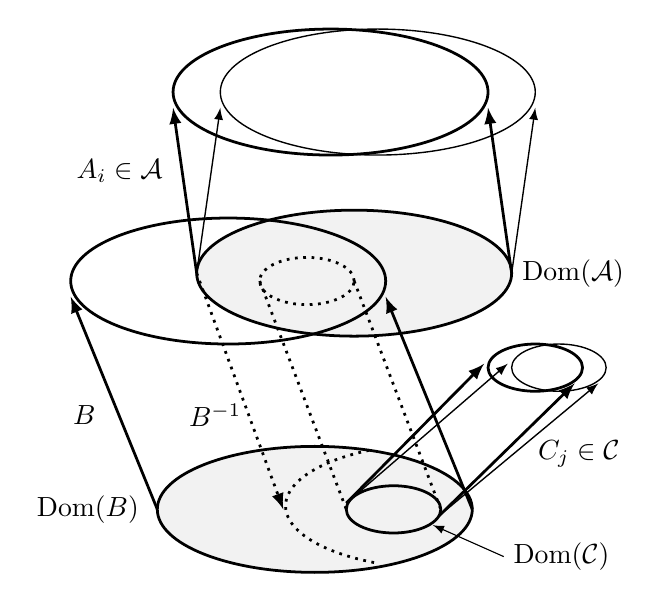
\begin{tikzpicture}
[line width=1pt]
\node at  (1.6+2, 0.1) [right] {$\textrm{Dom}(\seqset{A})$};
\draw[fill=black!5]     (1.6, 0.1) ellipse (2cm and 0.8cm); %% Dom A
\draw                   (1.3, 2.4) ellipse (2cm and 0.8cm); %% Img A1
\draw[line width=0.5pt] (1.9, 2.4) ellipse (2cm and 0.8cm); %% Img A2
\draw[-latex]                  (1.6+2, 0.1)--(1.3+2, 2.4-.2); %% A1 right
\draw[-latex]                  (1.6-2, 0.1)--(1.3-2, 2.4-.2); %% A1 left
\draw[-latex,line width=0.5pt] (1.6+2, 0.1)--(1.9+2, 2.4-.2); %% A2 right
\draw[-latex,line width=0.5pt] (1.6-2, 0.1)--(1.9-2, 2.4-.2); %% A2 left
\node at  (1.4-2-.1, 1.4) [left] {$A_i\in\seqset{A}$};
%%
\node at (1.1-2-.1, -2.9) [left] {$\textrm{Dom}(B)$};
\draw[fill=black!5] (1.1, -2.9) ellipse (2cm and 0.8cm); %% Dom B
\draw               (0  ,  0)   ellipse (2cm and 0.8cm); %% Img B
\draw[-latex] (1.1+2, -2.9)--(0+2, 0-.2); %% B right
\draw[-latex] (1.1-2, -2.9)--(0-2, 0-.2); %% B left
\node at  (0.55-2-.1, -1.7) [left] {$B$};
\draw[-latex,dotted] (1.6-2, 0.1)--(0.7, -2.9); %% B-1
\node at (0.3, -1.7) [left] {$B^{-1}$};
\draw[dotted] (1.79, -2.15) arc(118:244: 2cm and 0.8cm); %% Arc
\draw[dotted] (1, 0) ellipse (0.6cm and 0.3cm); %% Dotted S
\draw         (2.1, -2.9) ellipse (0.6cm and 0.3cm); %% Dom S
\draw[dotted] (1-0.6, 0)--(2.1-0.6, -2.9); %% B-1
\draw[dotted] (1+0.6, 0)--(2.1+0.6, -2.9); %% B-1
\draw                     (3.9, -1.1) ellipse (0.6cm and 0.3cm); %% Img S1
\draw[line width=0.5pt]   (4.2, -1.1) ellipse (0.6cm and 0.3cm); %% Img S2
\draw[-latex]                  (2.1-0.6, -2.9+.08)    --(3.9-0.6-.05, -1.1+.05); %% Left S1
\draw[-latex]                  (2.1+0.6-.02, -2.9-.08)--(3.9+0.6-.1, -1.1-.2); %% Right S1
\draw[-latex,line width=0.5pt] (2.1-0.6, -2.9+.08)    --(4.2-0.6-.05, -1.1+.05); %% Left S2
\draw[-latex,line width=0.5pt] (2.1+0.6-.02, -2.9-.08)--(4.2+0.6-.1, -1.1-.2); %% Right S2
\node at  (3.8,-2.2) [right] {$C_j\in\seqset{C}$};
\draw[-latex,thin] (3.5, -3.5) node[right]{$\mathrm{Dom}(\seqset{C})$} -- (2.1+0.5, -2.9-0.2);
\end{tikzpicture}\end{center}

\caption{Proof of \cref{r_invmove}}\label{fig_invmove}
\end{figure}

We see that the set of filesystems the sequences in $\seqset{A}$ do not break intersect with the range of $B$.
As $B$ is a bijection between its domain and range, we can use $B^{-1}$ to map this intersection back
onto the domain of $B$.
As $\worksc{B\cc \seqset{A}}{\seqset{C}}$ the domain of $\seqset{C}$ must be a subset of this
projected intersection.
If so, then we can use $B$ to map the domain of $\seqset{C}$, which yields the domain of $B^{-1}\cc \seqset{C}$.
As it is also a part of the domain of $A$, we get $\worksc{\seqset{A}}{B^{-1}\cc \seqset{C}}$.

The second part of the lemma can be proven in a similar way.
\end{proof}


\begin{mylem}\label{indep_prefix_combine}
The combination of sequences with a common head and independent tails 
continues to work under the same conditions:
\[ \worksc{A\cc B}{\seqset{S}} \wedge \worksc{A\cc C}{\seqset{S}} \wedge B\indep C \Rightarrow \worksc{A\cc B\cc C}{\seqset{S}} \]
\end{mylem}
\begin{proof}
Based on \cref{r_invmove} we know
$\worksc{B}{A^{-1}\cc \seqset{S}}$ and $\worksc{C}{A^{-1}\cc \seqset{S}}$,
and from \cref{combine_independent_sequences} we know
$\worksc{B\cc C}{B,C}$.
Combining these using \cref{workschained}
we get
$\worksc{B\cc C}{A^{-1}\cc \seqset{S}}$. 
Finally, applying the second line of \cref{r_invmove} yields
$\worksc{(A^{-1})^{-1}\cc B\cc C}{\seqset{S}}$, which proves our lemma 
as $\forall\FS: (A^{-1})^{-1}\aFS\typeeq A\aFS$ (\cref{negneg_is_typeeq}).
\end{proof}



\subsection{The Correctness of Reconciliation}

We are now ready to prove that the proposed algorithm for reconciliation is correct,
that is, applying its result is not going to break the replicas.
We reformulate the original proposition, $\reca\aFS_B\neq\fsbroken$,
based on $\FS_B=B\aFS$ and so we aim to prove that
$B\cc\reca$ works wherever $A$ and $B$ work:

\begin{myth}\label{reconciliation_correct}
If $A, B$ are simple, then $\worksmbb{A,B}{B\cc \reca}$,
where, to restate \cref{def:reconciliation},
\[ \reca = \{\alpha \whr \alpha\in \ambnp  \ \wedge\   \alpha\indep \bmanp \}. \]
\end{myth}

This is trivial unless $\worksmnilb{A,B}$, so we assume that it is true.
Let us first investigate the part of $A$ and $B$ that is excluded from
$\reca$: their intersection.

\begin{mylem}\label{can_move_intersection}
Let $A$ and $B$ be two simple sequences so that $\worksmnilb{A, B}$.
Then their intersection, in some suitable order, also works on any filesystem
either of them works on:
$\worksm{A}{\acbnp}$, and, by symmetry,
$\worksm{B}{\acbnp}$.
\end{mylem}

\begin{proof}
The difficulty is that commands in $\acbnp$ can occur anywhere in $A$.
Therefore, first we prove the following:
if all commands are marked in $A$ that also appear in $B$,
then there is an $A'$ in $\orderset{A}$ in which all marked commands are at the beginning.

We show that $A$ can be transformed via equivalences into $A'$ for which it is true.
Our proposition is that if the marked commands are not at the beginning, then
the sequence contains an unmarked command followed by a marked command.
We show that these can be swapped resulting in an equivalent sequence.
Then, by repeating this process similarly to bubble sorting, we can generate 
a suitable $A'$.

Let us consider therefore the marked command preceded by an unmarked command in $A$,
and let the marked command be $\cxynv$, 
and the preceding unmarked command be $\czwmv$:
\begin{gather*}
A = \cdots\cc  \czwmv\cc  \cxynv\cc  \cdots
\end{gather*}
As $A$ is simple and $\worksmnilb{A}$, from 
\cref{ax_distantrel_breaks,ax_directchild_breaks,ax_directparent_breaks}
we know that these commands can only be on incomparable nodes or form a construction or destruction pair.
In the first case, swapping the commands results in a sequence equivalent to $A$,
and we show that the last two cases are impossible as they would lead to contradiction.

In these cases, either $m=\parent(n)$ or $n=\parent(m)$.
If $B$ has a command on $m$, then
-- TODO TODO TODO --
from \cref{lemma:neighbor}
we know that there is a $B'$ in $\orderset{B}$ where it is next to $\cxynv$ (also in $B$),
and from \cref{simple_reorder_equiv} we know that $B'\equiv B$.
When describing our ordering algorithm in \cref{ordering} we saw
that the command on the parent path determines whether a pair of commands
is a construction or destruction pair,
and that this, in turn, determines whether the command on the child path must
precede or follow the other command as otherwise the sequence would break all filesystems.
This argument holds for both $A$ and $B$, and so the command on $m$ must be on
the same side of the command on $n$ in both sequences.

If $B$ has no command on $m$, then let $B'$ be $B$, 
but with an extra command added to it just before $\cxynv$
according to \cref{ax_child_assert,ax_parent_assert}, 
from which we know that $B'\equiv B$.
We also know that $B'$ is still minimal (but no longer simple).

In either case, therefore,
we have a minimal $B'$ which has a command on $m$ just before $\cxynv$ and $B'\equiv B$.
Let this command on $m$ be $\cqrmv$.
\begin{gather*}
A = \cdots\cc  \czwmv\cc  \cxynv\cc  \cdots \\
B' = \cdots\cc  \cqrmv\cc  \cxynv\cc  \cdots
\end{gather*}

As $\worksmnilb{A,B}$ and so $\worksmnilb{A,B'}$, 
from \cref{worksinputmatch}
we know that $[q]=[z]$. 

Going back to the construction and destruction pairs we see that the output value of the first command
is either $\vald$ or $\empt$ and is determined by the relationship between $n$ and $m$.
Therefore $r=w$ and $\cqrmv=\czwmv$.
If $B$ originally had a command on $m$,
this is a contradiction as $\czwmv$ was not marked, but we see it must also be in $B'$ and therefore in $B$.
If $B$ had no command on $m$,
this is a contradiction because the command on $m$ in $B'$ is an assertion command, so $[z]=[q]=[r]=[w]$, 
but $A$ contained no assertion commands.

We now know that there is an $A'\equiv A$ in which commands in $\acbnp$
are at the beginning, and therefore 
from \cref{worksextpostfix} we know that
$\worksm{A}{\acbnp}$ and by symmetry $\worksm{B}{\acbnp}$.
\end{proof}

\bigskip

\noindent
We would like to prove that $\worksmbb{A,B}{B\cc \reca}$.
From the above we know that we can move commands in $\acbnp$
to the beginning of $B$ and so this is equivalent to
\[ \worksmbb{A,B}{\acb\cc \bma\cc \reca}. \]
As we already know that $\reca\indep\bma$
and that $\worksmbb{A,B}{\acb\cc \bma}$
(as $\worksmbb{A,B}{B}$),
we can prove our theorem based on \cref{indep_prefix_combine}
if we can prove that
\[ \worksmbb{A,B}{\acb\cc \reca}. \]
Based on \cref{r_invmove} and \cref{repr_works_is_same}, and because
we already know that $\worksmbb{A,B}{\acbnp}$,
this is equivalent to
\[ \worksmbb{\acbi\cc A\T,\acbi\cc B\T}{\reca\T}. \]

To restate some results above, we therefore already know the following things:
\begin{itemize}
\item $\amb$ and $\bma$ are simple as $A$ and $B$ are simple
\item $\amb \cap \bma = \emptyset$
\item $\reca$ is the largest subset of $\amb$ for which $\reca\indep\amb$
\item $\worksmbb{\acbi\cc A,\acbi\cc B}{\amb, \bma}$ 
because of \cref{r_invmove}
as $\worksmbb{A,B}{A,B}$,
and $A\equiv\acb\cc\amb$, and $B\equiv\acb\cc\bma$.
\end{itemize}

Our theorem is therefore proven if we prove the following lemma,
in which we rename $\ambnp$ to $S$ and $\bmanp$ to $T$:
\newcommand{\condSimple}{(c1)}
\newcommand{\condDisj}{(c2)}
\newcommand{\condApr}{(c3)}
\newcommand{\condWork}{(c4)}
\begin{mylem}\label{reconciliation_correct_part}
If
   \begin{itemize}
   \item[\condSimple] $S$ and $T$ are simple sequences,
   \item[\condDisj] $S\cap T=\emptyset$,
   \item[\condApr] $S^*$ is the largest subset of $S$ where $S^*\indep T$, and
   \item[\condWork] $\worksmxb{\sqs{C}}{S,T}$ for some set of sequences $\sqs{C}$,
   \end{itemize}
then
\[ \worksmxb{\sqs{C}}{S^*}. \]
\end{mylem}

\begin{proof}
This is trivial unless $\worksmnil{\sqs{C}}$, so we will assume that it is true
and therefore $\worksmnilb{S,T}$.

The proof is similar to that of \cref{can_move_intersection}.
We mark all commands in $S$ that are in its subset $S^*$, and
we prove that $S$ can be transformed into $S'$ via equivalences
so that all marked commands would be at its beginning.
If so, then 
$\worksmxb{\sqs{C}}{S^*}$ 
based on \cref{worksextpostfix}
as $\worksmxb{\sqs{C}}{S'}$ and $S'=S^*\cc S_0$ 
where $S_0$ contains the remaining (conflicting) commands.

Again we know that if $S$ does not already have all marked commands at its beginning,
then there is an unmarked command followed by a marked one.
We show that these commands are independent and so they can be swapped
resulting in an equivalent sequence.
By repeating this process we can generate a suitable $S'$.

Let therefore the marked command in $S$ be $\cxynv$
and the preceding unmarked command be $\czwmv$.
As $S$ is simple and $\worksmnilb{S}$, from 
\cref{ax_distantrel_breaks,ax_directchild_breaks,ax_directparent_breaks}
we know that these commands can only be on incomparable nodes or form a construction or destruction pair.
In the first case, swapping the commands results in a sequence equivalent to $S$,
and we show that the other two cases are not possible as they would lead to a contradiction.

In the last two cases, we know that either $m=\parent(n)$ or $n=\parent(m)$.
We also know that because of {\condApr} there must be 
a command $\cqrov$ in $T$ which is not independent of $\czwmv$
as $\czwmv$ is not part of $S^*$.
\begin{gather*}
S = \cdots\cc  \czwmv\cc  \cxynv\cc  \cdots \\
T = \cdots\cc  \cqrov\cc \cdots
\end{gather*}
We know none of these commands is an assertion command, and 
from {\condDisj} that $\cqrov\neq\czwmv$.
Therefore, based on \cref{incomparable_is_independent} we know this means that
either $m\descendantEq o$ or $o\descendantEq m$.
From {\condApr} we also know that $\cxynv\indep \cqrov$,
and so because of \cref{incomparable_is_independent},
$n\unrel o$.

We therefore have four cases considering the relationships between $n,m$ and $o$:
\begin{itemize}
\item $n=\parent(m) \wedge o\descendantEq m$.
   This would mean that $o\descendantEq n$ or $n=\parent(o)$, which contradicts $n\unrel o$.
\item $n=\parent(m) \wedge m\descendantEq o$.
   This would mean that $n\descendant o$, which contradicts $n\unrel o$.
\item $m=\parent(n) \wedge o\descendantEq m$.
   This would mean that $o\descendant n$, which contradicts $n\unrel o$.
\item $m=\parent(n) \wedge m\descendantEq o$.
   Let us continue with this case.
\end{itemize}

We know that $T$ cannot have a command on $m$ as $m=\parent(n)$ and $\cxynv\indep T$,
and so $m\neq o$ and therefore $m\descendant o$.
This means we can create a new sequence $T'\equiv T$ by inserting a command on 
$m$ into $T$ before $\cqrov$
according to \cref{ax_parent_assert}.
We now have $\cxynv\indep T\equiv T'$, which is a contradiction as
$T'$ has a command on $m$ and $m=\parent(n)$.
\end{proof}



\subsection{The Completeness of Reconciliation}

% Reconciliation is maximal
% -------------------------
% This is where we're using |D|=1

The reconciliation algorithm defined above is also complete, that is,
it is not possible to apply any further commands from $A\setminus B$ to $\FS_B$.
To show this, we are going to prove the following \namecref{rec_is_complete}:

\begin{myth}\label{rec_is_complete}
If $A$ and $B$ are simple sequences,
and we select a sequence $S\subset \amb$ so that
it contains a command $\cxynv$ for which $\cxynv\nindep\bma$,
then $B\cc S$ either breaks all filesystems $A$ and $B$ do not break
(that is, $S$ breaks all possible $\FS_B$ replicas),
or it changes a node that $B$ has already changed to a different value,
that is, it overrides a change in $\FS_B$.
\end{myth}
Such an override could occur if a given node was modified differently in
$A$ and $B$ (to different values but the same type), which is clearly
a conflict that should be marked for review
by a human or a different system.
\begin{proof}
The proof is similar to the ones we have seen above.
Without loss of generality, we assume that $\cxynv$ is the first command in $S$
that is not independent of $\bma$.
If so, we can split $S$ into $S_0\cc\cxynv\cc S_1$ where $S_0\indep\bma$.
Let us also split $\bma$ into $T_0\cc\czwmv\cc T_1$ where $T_1\indep\cxynv$.
From \cref{can_move_intersection} we know that
$B\cc S \equiv \acb\cc\bma\cc S$.
We also know that commands in $S_0$ and $\bma$ commute, and so this is equivalent to
$\acb\cc S_0\cc\bma\cc\cxynv\cc S_1$.
Expanding $\bma$ and swapping $T_1$ and $\cxynv$ we get
\[ \acb\cc S_0\cc T_0 \cc \czwmv \cc \cxynv\cc T_1\cc S_1. \]

First, we prove that this sequence breaks all filesystems
unless $n=m$.
Let us therefore suppose $n\neq m$ and, to use an inverse proof,
that the sequence works on $\FS$ where $A\FS\neq\fsbroken$.
If so, its initial segment, $\acb\cc S_0\cc T_0 \cc \czwmv \cc \cxynv$ must also work.

We know $\cxynv\nindep\czwmv$, and so from \cref{incomparable_is_independent}, $n\nunrel m$.
As the sequence works, $\czwmv\cc\cxynv$ can only be a construction or destruction pair.
As $\czwmv$ and $T_0$ originate from $B\setminus A$ and $B$ is simple, we also know there are
no commands on $m$ in $A\cap B$ or $T_0$,
and that there are no commands on $m$ in $S_0$ as $S_0\indep\bma$.

On the one hand we therefore know that $\FS(m)$ must be of type $Z$,
but on the other, from \cref{ax_directchild_breaks,ax_directparent_breaks},
we also know that $\cxynv$ cannot be applied to $\FS$ without
changing $\FS(m)$ first.
As $A\FS\neq\fsbroken$, this means that $A$ must contain a command on $m$.
Let this command be $\cqrmv$.

Clearly $Q=Z$ (from \cref{worksinputmatch}), and from the construction and destruction
pairs we also see that $R=W$ must hold, where $W=\cchard$ or $W=\ccharb$.
As $|\setd|=1$ and $|\setb|=1$, this also means that $v_R=v_W$ and therefore
$\cqrmv = \czwmv$.
This is a contradiction as $\cqrmv\in A$, but $\czwmv\in\bma$.

The only possibility is therefore $n=m$.
As $A$ and $B$ are simple, we therefore know that these are the first commands on $n$,
and so (again from \cref{worksinputmatch}) $Z=X$.
We also know $\valvw\neq\valvy$ as otherwise the two commands would be equal and
would be included in $A\cap B$,
but this means that $\cxynv$, from $A$, overrides a change introduced 
by $\czwnv$, from $B$, which should be treated as a conflict.
\end{proof}

From the proof it is apparent that this result depends on $|\setd|=1$.



% section

\section{Related Work}

\subsection{Liberal and Conservative Reconciliation}

We consider the reconciliation algorithm described here an improvement over
the one derived during our previous research \cite{NREC}
as the previous algorithm not only fails to propagate all possible commands
wherever it is possible (that is, where it does not break the filesystem),
but the current algorithm is also simpler.
This is because the previous reconciliation algorithm excludes
commands from being propagated which must be preceded by a command that conflicts.

The former observation is supported by Berzan and Ramsey, who in \cite{CBNR} 
describe different general reconciliation policies.
The liberal (maximal) policy propagates all updates to all replicas where
the update does not break the filesystem, while a conservative policy
refrains from updating any node that is below a node with conflicting commands.
They show that the reconciliation algorithm in \cite{NREC} implements
an intermediate policy as one can easily construct two- or three-replica scenarios
where an update could clearly be propagated, but it is excluded.
To rephrase the example in \cite{CBNR}, consider the following two
update sequences that have been applied to replicas $\FS_A$ and $\FS_B$:
\begin{align*}
A&=\caaa{\empt}{\valdi}{\nn}\cc\caaa{\empt}{\valf}{n} \\
B&=\caaa{\empt}{\valdii}{\nn}
\end{align*}
where $\parent(n)=\nn$ (\cite{NREC} did not require all directories to have the same value).
Clearly $\caaa{\empt}{\valf}{n}$ could be applied to $\FS_B$, but it is not as
it must be preceded by creating the directory, which conflicts with the same command in $B$
due to the different value.
(Introducing a third replica which has not changed at all further complicates the picture.)
The current algorithm no longer needs to specify that there can be no conflicts
on preceding commands, and, to use the above terminology, implements a fully liberal policy.


\subsection{Comparing Definitions of Conflicts}

As a test of the proposed reconciliation algorithm, 
we compare our definition of conflicting
updates to how conflicts are defined by Balasubramaniam and Pierce
in their state-based approach implemented in the Unison synchronizer \cite{BP}.
As we noted in \cite{NREC}, the update detector they describe provides a safe estimate of nodes
(paths) at which updates occurred.
It marks some nodes as \emph{dirty} in a way that we know that at non-dirty nodes
the filesystems (replicas) have not changed between their common original state and current state
(see Definition 3.1.1 in \cite{BP}).
The \emph{dirty} marks are also up-closed, that is, all ancestor nodes of a dirty node
are also dirty (Fact 3.1.3 in \cite{BP}).
And finally, in our notation, 
a conflict is detected between replicas $\FS_A$ and $\FS_B$ at node $n$
if $n$ is marked as dirty in both $\FS_A$ and $\FS_B$, and
$\FS_A(n)\neq\FS_B(n)$, and $n$ does not point to a directory in both replicas.
(In other words, 
$\FS_A(n)\not\in\setd \vee \FS_B(n)\not\in\setd$; see section 4.1 in \cite{BP}.
Let us note that there is an alternative approach to defining an algorithm for
the same synchronizer by Pierce and Vouillon in \cite{PV}.)

It can be easily seen that due to an edge case, 
not all conflicts detected based on the above definition
entails a conflict based on our system; that is, \cite{BP} describes a more
conservative policy.
We use the example we described in \cite{NREC},
where $\nn=\parent(n)$ and $\FS(\nn)$ is a directory and $\FS(n)$ is a file, and
the two replicas are derived in the following way:
\begin{gather*}
\FS_A = \cfba{n} \cc \cdba{\nn} \aFS \\
\FS_B = \cfba{n} \aFS.
\end{gather*}
Then, $\nn$ is dirty in both replicas:
in $\FS_A$ it was modified, and in $\FS_B$ one of its descendants was modified.
Moreover, $\FS_A(\nn)\neq\FS_B(\nn)$ and $\FS_A(\nn)=\empt\not\in\setd$,
and therefore a conflict is detected at $\nn$.
(This behaviour is preserved in the more recent Harmony synchronizer.
See ``delete/delete conflicts'' in \cite{PSG,FGKPS}.)
Our reconciliation algorithm detects no conflicts;
instead, it propagates $\cdba{\nn}$ to $\FS_B$, which we think is as expected
and desired.

At the same time, it can be shown that if our command-based reconciler
detects a conflict, it entails a conflict in the state-based reconciler.
We note here that Balasubramaniam and Pierce also suppose that all directories are equal,
therefore, as elsewhere, we are safe to continue to assume that $|\setd|=1$.

\begin{proof}
Let $A$ and $B$ be two simple sequences returned by the update detector
for the two replicas $\FS_A$ and $\FS_B$.
A conflict between the commands $\cxynv\in A$ and $\czwmv\in B$
means that even though $\cxynv\in A\setminus B$
and $\czwmv\in B\setminus A$, they cannot be included in
$\reca$ and $\recb$, respectively, because
$\cxynv\nindep\czwmv$ (see \cref{def:reconciliation}).

From \cref{incomparable_is_independent} we therefore know that $n\nunrel m$.
Without loss of generality we can assume that $n\descendantEq m$.
From this we see that $n$ is \emph{dirty} in both $\FS_A$ and $\FS_B$,
as the filesystem changes at $n$ in $\FS_A$ and at $n$ or its descendant in $\FS_B$
(and none of the commands are assertion commands).

Now we only need to show that $\FS_A(n)\neq\FS_B(n)$, because from this 
and $|\setd|=1$ we will also
know that at least one of these values is not a directory,
and therefore there is a conflict at $n$ in the state-based reconciler.
If $n=m$, this follows from the fact that $\cxynv\neq\czwmv$ 
(because they are not in $A\cap B$),
as from \cref{worksinputmatch} we have $X=Z$,
and therefore the above can only be true
if $\FS_A(n)=\valvy\neq\valvw=\FS_B(n)$.
If $n\descendant m$ and there is no command on $n$ in $B$, then it is also
true as $\cxynv$ is not an assertion command, and therefore 
$\FS_A(n)\neq\FS(n)=\FS_B(n)$, where $\FS$ is the common ancestor of the replicas.
Finally, if there is a command on $n$ in $B$, then 
from $\cxynv\in A\setminus B$ we know
it must be different from $\cxynv$, and similarly to the first case,
we have $\FS_A(n)\neq\FS_B(n)$.
\end{proof}



% section

\subsection{Towards an Algebra}\label{sec_algebra}

Similarly to \cite{NREC} we can consider creating an algebra over command sequences
which will enable us to draw conclusions about the behaviours of the sequences
independently of filesystems.
This would provide a secondary model of (filesystem) commands above the model a filesystems
defined in this paper. The new model would no longer describe filesystems as such,
but use known relationships between sequences of commands as its starting point.

In this algebra, equivalence ($\equiv$) and extension ($\eqext$) would become relations,
and logical rules involving them
(e.g. $ A\equiv B \Rightarrow S\cc A\cc T\equiv S\cc B\cc T $) would be re-cast as inference rules.
In addition to these, the \namecrefs{ax_separate_commute} listed in \cref{section_axioms}
would become axioms that we accept as true, and from which other true statements can be derived
using the inference rules.
Such a system can allow us to deduce, for example, whether two sequences are equivalent
or one extends the other
without reference to filesystems.

We note, however, that the \namecrefs{ax_separate_commute} to be used as axioms 
specify the relationships between the nodes
the commands act on, which would require a more complicated set of symbols to represent
in the algebra.
To avoid this, we think it will be more fruitful to regard commands (and sequences)
on different nodes as different, and, in effect, have nine times as many commands 
in the algebra as there are nodes in the namespace of the filesystems.
This allows us to reduce the number of types of symbols in our algebra, and regard
the \namecrefs{ax_separate_commute} not as axioms, but as templates for axioms
from which all axioms (for pairs of separate nodes, etc.) can be generated.

We expect that the soundness and completeness of such an algebra can be proven
similarly to the proofs described in \cite{NREC}.
Indeed, results in the current paper can serve as building blocks of such a proof:
the computer program used to check the \namecrefs{ax_separate_commute}
in effect proves the soundness of all axioms,
and \cref{simple_reorder_equiv} proves completeness in a limited sense.
It is also worth noting that the majority of proofs presented in this paper
do not actually refer to specific filesystems or the definition of commands,
but draw on known relationships and the
\namecrefs{ax_separate_commute} in \cref{section_axioms}.
In other words, many proofs are transferable to the algebra that we describe here.

In a more complete algebra from which the correctness and completeness
of reconciliation could also be derived,
one can also include symbols, inference rules and axioms for 
$\works{\seqset{X}}$ and $\worksc{\seqset{X}}{\seqset{Y}}$.
We see proving the soundness and completeness of this extended algebra
an intriguing problem that is worthy of further research.


% section
%% Conclusion
\section{Conclusion}

We built an algebra of commands on filesystems. Then we proved that the
algebra is sound and complete, that is, commands which are algebraically
equivalent commands are also equivalent on real filesystems, and vice
versa.

We defined conflicts with the help of this algebra, then we defined
algorithms for update--detection and reconciliation. Finally, we
implemented these algorithms and tested it on numerous cases (see
Appendix \ref{app:impl}). The results were always in accordance with what
we expected from the philosophy ``propagate every command possible on
every replica''.  Because of that, using algebraical methods in file
synchronization turned out to be an effective solution.

We also gained some information about the provability of such theorems and
algebras. The methods we used in the proofs are likely be able to be used
in proofs for other algebras as well, so that we would be able to create a
more general theory of synchronization.




\section{Acknowledgments}

I thank Laszlo Csirmaz for his invaluable input on this paper,
and Bill Zissimopoulos for his observations on algebraic file synchronization that triggered this research.

\begin{thebibliography}{99}


\bibitem{NREC} 
Norman Ramsey and Elod Csirmaz,
``An Algebraic Approach to File Synchronization,''
in \emph{Proceedings of the Joint 8\textsuperscript{th} European Software Engineering Conference 
and 9\textsuperscript{th} ACM SIGSOFT Symposium on the Foundations of Software Engineering,}
New York: ACM, 2001, pp. 175--185.

\bibitem{CBNR} 
Constantin Berzan and Norman Ramsey,
``Summer Scholars Technical Report,''
Medford, MA: Tufts University, 2010.
Accessed 29 November 2015.
http://thirld.com/files/summerscholars\_techreport.pdf.

% 5
\bibitem{TTPDSH}
% D. B. Terry and M. M. Theimer and Karin Petersen and A. J. Demers and M. J. Spreitzer and C. H. Hauser
D. B. Terry et al.,
``Managing Update Conflicts in Bayou, a Weakly Connected Replicated Storage System,''
in \emph{Proceedings of the Fifteenth ACM Symposium on Operating Systems Principles,}
New York, NY: ACM, 1995, pp. 172--182.


% 4
\bibitem{BP}
S. Balasubramaniam and Benjamin C. Pierce,
``What is a File Synchronizer?''
in \emph{Proceedings of the 4\textsuperscript{th} Annual 
ACM/IEEE International Conference on Mobile Computing and Networking,}
New York: ACM, 1998, pp. 98--108.


% 3
\bibitem{KRSD}
Anne-Marie Kermarrec and Antony Rowstron and Marc Shapiro and Peter Druschel,
``The IceCube Approach to the Reconciliation of Divergent Replicas,''
in \emph{Proceedings of the Twentieth Annual ACM Symposium on Principles of Distributed Computing,}
New York: ACM, 2001, pp. 210--218.


\end{thebibliography}

\end{document}
